\documentclass[oneside,12pt,a4paper,headsepline,bibtotocnumbered]{memoir}
%\documentclass[oneside,12pt,a4paper]{memoir}
%\documentclass[a4paper,12pt,twoside,headsepline,pointlessnumbers,bibtotocnumbered]{scrbook}

\usepackage[utf8]{inputenc}
\usepackage{graphicx}
%\usepackage{lettrine}
\usepackage{hyperref}
\usepackage{color}
\usepackage{url}

\usepackage[T1]{fontenc}
\usepackage{lmodern}
%\usepackage{psfig}
%\usepackage{psfrag}
%\usepackage{epsfig}
\usepackage{epstopdf}
% Formato de paquetes de SCTP y NALUs de SVC...
%\usepackage{bytefield}
% Algoritmos
%\usepackage{algorithm}
%\usepackage{algpseudocode}
% Columnas
\usepackage{multicol}
\usepackage[labelfont=bf]{caption}
% Listados
\usepackage{listings}
\usepackage{pdfpages}
\usepackage{indentfirst}
\usepackage[official]{eurosym}


%euro
%\usepackage{eurosym}

%\usepackage[bookmarks = true, colorlinks=true, linkcolor = black, citecolor = black, menucolor = black, urlcolor = black]{hyperref}

%\newsubfloat{figure}% Allow subfloats in figure environment

%\usepackage{wrapfig}

\usepackage{listings}
%\usepackage[usenames,dvipsnames]{xcolor}

\definecolor{gray97}{gray}{.97}
\definecolor{gray75}{gray}{.94}
\definecolor{gray45}{gray}{.45}
\definecolor{verde}{RGB}{230,255,204}

\usepackage{listings}

\newcommand\Tstrut{\rule{0pt}{2.6ex}}       % "top" strut
\newcommand\Bstrut{\rule[-0.9ex]{0pt}{0pt}} % "bottom" strut
\newcommand{\TBstrut}{\Tstrut\Bstrut} % top&bottom struts


\newenvironment{filecode}[1][]
  {\minipage{\linewidth}% \begin{filecode}[#1]
   \lstset{basicstyle=\ttfamily\footnotesize,frame=single,#1}}
  {\endminipage}% \end{filecode}


%\DeclareInputText{128}{\euro}

\definecolor{azulillo}{rgb}{0.8,0.85,1}
\definecolor{marronrp3}{rgb}{.9,.9,.7}
\definecolor{salmon}{rgb}{1,.9,.8}
\definecolor{rojo}{rgb}{.8,0.1,.0}
\definecolor{rojo2}{rgb}{.6,0.3,.2}

\lstset{
  basicstyle=\ttfamily,
  columns=fullflexible,
  showstringspaces=false,
  commentstyle=\color{gray}\upshape
}

\lstdefinelanguage{XML}
{
  morestring=[b]",
  morestring=[s]{>}{<},
  morecomment=[s]{<?}{?>},
  stringstyle=\color{black},
  identifierstyle=\color{darkblue},
  keywordstyle=\color{cyan},
  morekeywords={xmlns,version,type}% list your attributes here
}

\lstdefinestyle{BashInputStyle}{
  language=bash,
  basicstyle=\small\sffamily,
  numbers=left,
  numberstyle=\tiny,
  numbersep=3pt,
  frame=tb,
  columns=fullflexible,
  linewidth=0.9\linewidth,
  xleftmargin=0.1\linewidth,
  commentstyle=\color{dkgreen},
}

\definecolor{dkgreen}{rgb}{0,0.6,0}
\definecolor{gray}{rgb}{0.5,0.5,0.5}
\definecolor{mauve}{rgb}{0.58,0,0.82}

\lstset{frame=tb,
  language=Java,
  aboveskip=3mm,
  belowskip=3mm,
  showstringspaces=false,
  columns=flexible,
  basicstyle={\small\ttfamily},
  numbers=none,
  numberstyle=\tiny\color{gray},
  keywordstyle=\color{blue},
  commentstyle=\color{dkgreen},
  stringstyle=\color{mauve},
  breaklines=true,
  breakatwhitespace=true
  tabsize=3
}


\def\changemargin#1#2#3{\list{}{\rightmargin#2\leftmargin#1\headsep#3}\item[]}
\let\endchangemargin=\endlist


%\configuracion{TituloDocumento}{TextoEncabezadoIzdo}
\newcommand{\configuracion}[2]{
	\renewcommand{\shorthandsspanish}{}
	\title{#1}
	\date{}
	\evensidemargin -6mm  \oddsidemargin -0.4cm \textwidth 16.7cm
	\usepackage[colorlinks=true,linkcolor=blue,urlcolor=blue]{hyperref}
	\textheight 24cm \topmargin -0.65cm
	\pagestyle{fancy}
	\lhead{#2}
	\rhead{\thepage}
	\cfoot{}
}

\newcommand{\escudos}{
	\begin{changemargin}{-1.0cm}{-3cm}{0cm}
		\begin{flushleft}
  			\begin{figure}
    			
\includegraphics[scale=0.2]{escudo.jpg}
    			\hspace*{8cm}
    			\includegraphics[scale=0.45]{informatica.png}
    		\end{figure}
		\end{flushleft}
	\end{changemargin}
}

\newcommand{\asignatura}[1]{
	\begin{center}
#1
	
	\end{center}
}

\newcommand{\titulacion}[1]{
	\begin{center} 
	#1
	\end{center} 
}

\newcommand{\cursiva}[1]{
	\textit{#1}
}

\renewcommand{\bibname}{References}

%%%%%%%%%%%%%%%%%%%%%%%%%%%%%%%%%%%%%%%%%%%%%%%%%%%%%%%%%
% \shadowbox{Texto}: Marco sombreado. 
%\ovalbox{Texto}: Marco ovalado. 
%\doublebox{Texto}: Marco doble. 
% \Ovalbox{Texto}. Marco ovalado. 


% \cajaBorde {texto}{color letra}{color fondo}
\newcommand{\cajaBorde}[3]{
	\noindent
	\fcolorbox{#2}{#3}{
  		\begin{minipage}[t]{.96\linewidth}
   			 \vspace{.05cm}
    		\begin{center}
     			 \vspace{.1cm}
     			#1
   			 \end{center}
 		 \end{minipage}
	}
}

%caja{texto}{color caja}{espacio superior}{espacio inferior}
\newcommand{\caja}[4]{
	\colorbox{#2}{
 	 \begin{minipage}[t]{.96\linewidth}
 	 \vspace{#3}
  		
			#1
		
   	 \vspace{#4}
 	 \end{minipage}
	}
}

\newcommand{\borde}[1]{\framebox{#1}}

%\portada{asignatura}{pratica}{tituloCaja}{titulacion}{autores}
\newcommand{\portada}[5]{
	%PORTADA
	\thispagestyle{empty}

	%Escudo universidad
	\escudos

	\LARGE

	\asignatura{#1}

	\vspace*{0.8cm}

	\begin{center}
		\textbf{#2} %Práctica 1\\
	\end{center}


	\begin{center}

		
	\colorbox{azulillo}{
 	 	\begin{minipage}[t]{.96\linewidth}
 	 		\vspace{.5cm}
  		
			\begin{center}
				\textbf{#3}
			\end{center}
		
   	 		\vspace{.02cm}
 		\end{minipage}
	}		
		
	\end{center}

	\Large
	\vspace {3cm}

	\titulacion{#4}

	%Fecha
	\begin{center}
		\today
	\end{center}
	\normalsize
	\vspace*{2cm}

	\begin{flushright}
		#5
	\end{flushright}

}

%\portada{asignatura}{pratica}{tituloCaja}{titulacion}{autores}
\newcommand{\portadaumu}[5]{
	%PORTADA
	\thispagestyle{empty}
\setlength{\unitlength}{1 cm} %Especificar unidad de trabajo
\thispagestyle{empty}
\begin{picture}(18,4)
\put(0,0){
\includegraphics[scale=0.33]{escudo.jpg}}
\put(11.5,0){\includegraphics[scale=0.43]{informatica.png}}
\end{picture}
\\
\\
\begin{center}
\textbf{{\Huge University Charles III}\\[0.5cm]
{\LARGE Faculty of Computer Science}}\\[1.25cm]
\Large #1\\[2cm]


\LARGE \textbf{#3}\\[0.3cm]

{\large #5}\\[1.6cm]
#4\\[1cm]
Madrid - \today
\end{center}

}

\newcommand{\indice}{

	\newpage
	\setcounter{page}{1}
	\renewcommand{\thepage}{\roman{page}}
	\tableofcontents
	\newpage
	\clearpage
	\setcounter{page}{1}
	\renewcommand{\thepage}{\arabic{page}}
}


\lstset{basicstyle=\small\ttfamily,showstringspaces=false,language=sh,frame=tb,columns=fullflexible}

% Separación entre párrafos
%\setlength{\parindent}{0pt}
% %\nonzeroparskip
\usepackage{lscape}

\usepackage[table,xcdraw]{xcolor}
\usepackage{listings}
% Veelo un poco cambiado


\usepackage{pgfgantt}

\usepackage{geometry}
\geometry{
	left=30mm,
	right=30mm,
	top=25mm,
}

\definecolor{barblue}{RGB}{153,204,254}
\definecolor{groupblue}{RGB}{51,102,254}

\makeatletter
\newlength{\numberheight}
\newlength{\barlength}
\makechapterstyle{myveelo}{%
\setlength{\beforechapskip}{40pt}
\setlength{\midchapskip}{25pt}
\setlength{\afterchapskip}{40pt}
\renewcommand{\chapnamefont}{\normalfont\LARGE\flushright}
\renewcommand{\chapnumfont}{\normalfont\HUGE}
\renewcommand{\chaptitlefont}{\normalfont\HUGE\bfseries\flushright}
\renewcommand{\printchaptername}{%
\chapnamefont\MakeUppercase{\@chapapp}}
\renewcommand{\chapternamenum}{}
\setlength{\numberheight}{18mm}
\setlength{\barlength}{\paperwidth}
\addtolength{\barlength}{-\textwidth}
\addtolength{\barlength}{-\spinemargin}
\renewcommand{\printchapternum}{%
\makebox[0pt][l]{%
\hspace{.4em}%
\resizebox{!}{\numberheight}{\chapnumfont \thechapter}%
%\hspace{.8em}%
%\rule{\barlength}{\numberheight}
}}
\makeoddfoot{plain}{}{}{\thepage}
}
\makeatother

% Configuración de márgenes más anchos
\setmarginnotes{0pt}{0pt}{0pt}
\settypeblocksize{675pt}{450pt}{*}
\setlrmarginsandblock{2.7cm}{2.7cm}{*}
\setulmarginsandblock{2.7cm}{2.7cm}{*}
\checkandfixthelayout
\raggedbottom

\chapterstyle{myveelo}

% Numeración de subsecciones
\setcounter{secnumdepth}{2}

\newcommand{\first}[2]{
%lhang=1, nindent=0pt, 
	\lettrine[lines=3]{#1}{#2}%
}

\newcommand{\figura}[4]{%
    \begin{figure}[ht]
    \begin{center}
	    \includegraphics[#2]{#1}
	    \caption{#3}
	    \label{#4}
    \end{center}
    \end{figure}
}


\begin{document}
	
	\newcommand{\HRule}{\rule{\linewidth}{0.5mm}}

\begin{titlingpage}
\begin{center}
 
% Upper part of the page
\vfill

\includegraphics[scale=1.2]{./images/escudo}\\[3em]
\textsc{\LARGE Universidad Carlos III de Madrid}\\[0.5cm]
\textsc{\Large Trabajo de Fin de Grado}\\[0.5cm]

% Title
\HRule \\[0.6cm]
\textbf{\Large Integration of CROWD SDN-based DMM solution with NI PXI Systems for LTE emulation}
\HRule \\[0.6cm]
 
% Author and supervisor
\begin{minipage}{0.45\textwidth}
\begin{flushleft} \large
\emph{Student:}\\
Jason \textsc{Moorcroft}\\ jmoorcr@it.uc3m.es
\end{flushleft}
\end{minipage}
\begin{minipage}{0.45\textwidth}
\begin{flushright} \large
\emph{Tutor:} \\
Antonio \textsc{De la Oliva}\\
aoliva@it.uc3m.es
\end{flushright}
\end{minipage}
 
\vfill
 
% Bottom of the page
{\large \today}
 
\end{center}

\end{titlingpage}
	
	\clearpage\null\newpage
	
	%Acknowledgments:
\textsc{\Large Acknowledgments}\\[0.5cm]


This project marks the end of an amazing part of my life, I wouldn't have been able to achieve it without the help of many people.\\

First of all, thanks to my family for supporting me the whole way and making  me feel like anything with hard work can be achieved. Thanks to those words, I have found the strength to not give up even when I thought I wasn't capable of accomplishing what I set out to do.\\

To my partner Maria, thank you so much for making this journey by me, for being there to help me without asking and for making this stage of my life as amazing as it has been. \\

To "Mis Costillas", for making those long afternoons in the library and in class so much more interesting. For the amazing places we have visited throughout these years, thank you.\\

Thank you to my friends for being understanding and helping me disconnect from the long days at university and show me a good time.\\

Thanks to my tutors,Pablo and Carlos, for guiding me through this project and showing interest in helping me express my ideas.\\
















	
	\clearpage\null\newpage
	\clearpage{\cleardoublepage}
	
	\makepagestyle{init}
	   \makeevenfoot{init}{\thepage}{}{}
	   \makeoddfoot{init}{}{}{\thepage}
	   \makeevenhead{init}{}{}{}
	   \makeoddhead{init}{}{}{}
	   \makeheadrule{init}{0pt}{0pt}
	
	\pagestyle{init}
	  \tableofcontents*\thispagestyle{init}
	  \clearpage
	  \listoffigures*\thispagestyle{init}
	  \clearpage
	  \listoftables*\thispagestyle{init}
	\clearpage\null\newpage
  	\chapter*{Abstract}
\addcontentsline{toc}{chapter}{Abstract}

The lack of expertise that people have on how to perform a good training session, leads to inefficiency and bad practices that can lead people to quit or injure themselves. With the cost to have a personal trainer or somebody to manage a persons training session being very high, there is an opportunity to improve the user experience with automated services that provide relevant information and keeps track of the progress that is being made.\\

This project implements a trainer chat bot that alleviates the cost of having a personal trainer, but maintaining many of the features they would provide. Over the years chat bots have steadily been incorporated into society, the flexibility and cost chat bots have, makes a very lucrative option for monotonous operations such as some provided by a personal trainer. 






	\clearpage
	\clearpage\null\newpage

	\pagestyle{ruled}
  
  	\chapter{Introduction}\label{chap:1}
Technology and the impact it is having in our society is changing the way we think and the way we interact with each other. With more and more automation in the workplace many monotonous jobs are disappearing and more creative ones are replacing them. This and the fact that technology has opened the mind and ability for people to start a business as the cost to startup a business thanks to technology has greatly reduced.
The objective of this project is to automate the personal training area as it has been relatively untouched. The problem is that many people unknowingly train in a way that in the long term may cause them injury, this is due to the lack of knowledge and guidance to train differently and safely. Gym trainers may provide some guidance but with the amount of people normally in these gyms they can’t be always there to help. The idea is to create a chatbot that can aid, track progress and create training sessions that adapt to each user whenever the user needs them. 
\section{Background}\label{sec:chap1_background}
Machine Learning (ML) algorithms in recent years have improved greatly thanks to the immense computing power available. This with the amount of data currently accessible, has naturally led the way for the development of bots that can communicate with people, originally with basic phrases and over time in a more complex and natural manner. New technologies have made it more intuitive and easier to work on this area with many Natural Language Processing (NLP) libraries such as Natural Language Tool Kit (NLTK) that help translate human spoken phrases to something easier for the computer to understand. Other libraries like TensorFlow or Scikit-Learn provide functionality to train models based on the processing done in NLTK.
Nowadays, even though the libraries mentioned before are still frequently used, it is more common now to see platforms that abstracts the users from the inner workings of the algorithms and instead leaves the user with an intuitive UI for the user to create their own functionality for the chatbot.

Thanks to the access we have now to smartphones and social platforms the integration of chatbots in these platforms is growing steadily as it allows the user to communicate with help centers without waiting a long time to get a response.

\section{Motivation}\label{sec:chap1_moti}
The motivation to develop this project comes from the time-consuming activity of preparing a time table with what muscles and exercises to train and the forgetful way of tracking a person’s progress when going to the gym, for this reason, with the knowledge acquired over the years and the technology available this project came to life. It is not only a project to finish the degree it is a project that after giving it in will still be worked on over time to add more functionality and make it a truly useful application that can be used by users outside the University environment. This will be more of a proof of concept to verify the viability of further developing and investing the time to add more functionality.

\subsection{Survey}\label{sec:chap1_reas_app}

To prove that the application has a market opportunity an inquire was made to a group of people with over 200 people, the results where interesting as will be explained below. The language of the form is in Spanish as the public inquired live in Spain.\\

As shown below most of the users filling the form are from age 16 to 25, this gives context to some of the answers given afterwards, in this case generational mentality plays an important role as different age groups may have a different opinion on gym training. In this case the target group even though available for every age group is more focused on people in those age limits as they are the most common at gyms, the least informed and the more friendly with technology they are.

\begin{center}
	\begin{figure}[h!]
		\centering
		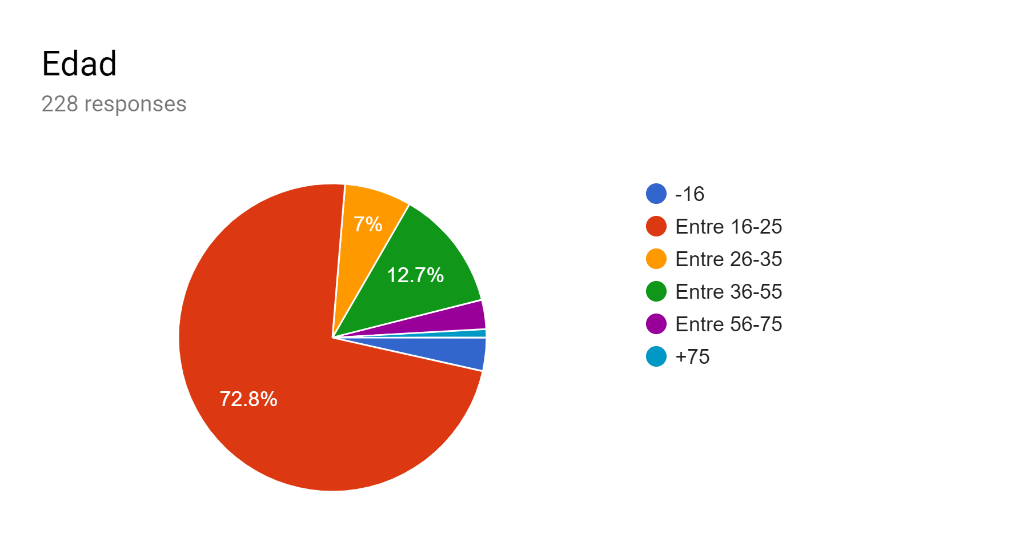
\includegraphics[scale=1]{./images/4-age}
		\caption{Survey: Age}
		\label{4_age}
	\end{figure}
\end{center}

In the case of gender, the pool has been varied with close to 50\% of each gender, this with the age group gives a general perception of what people think of the questions asked.

\begin{center}
	\begin{figure}[h!]
		\centering
		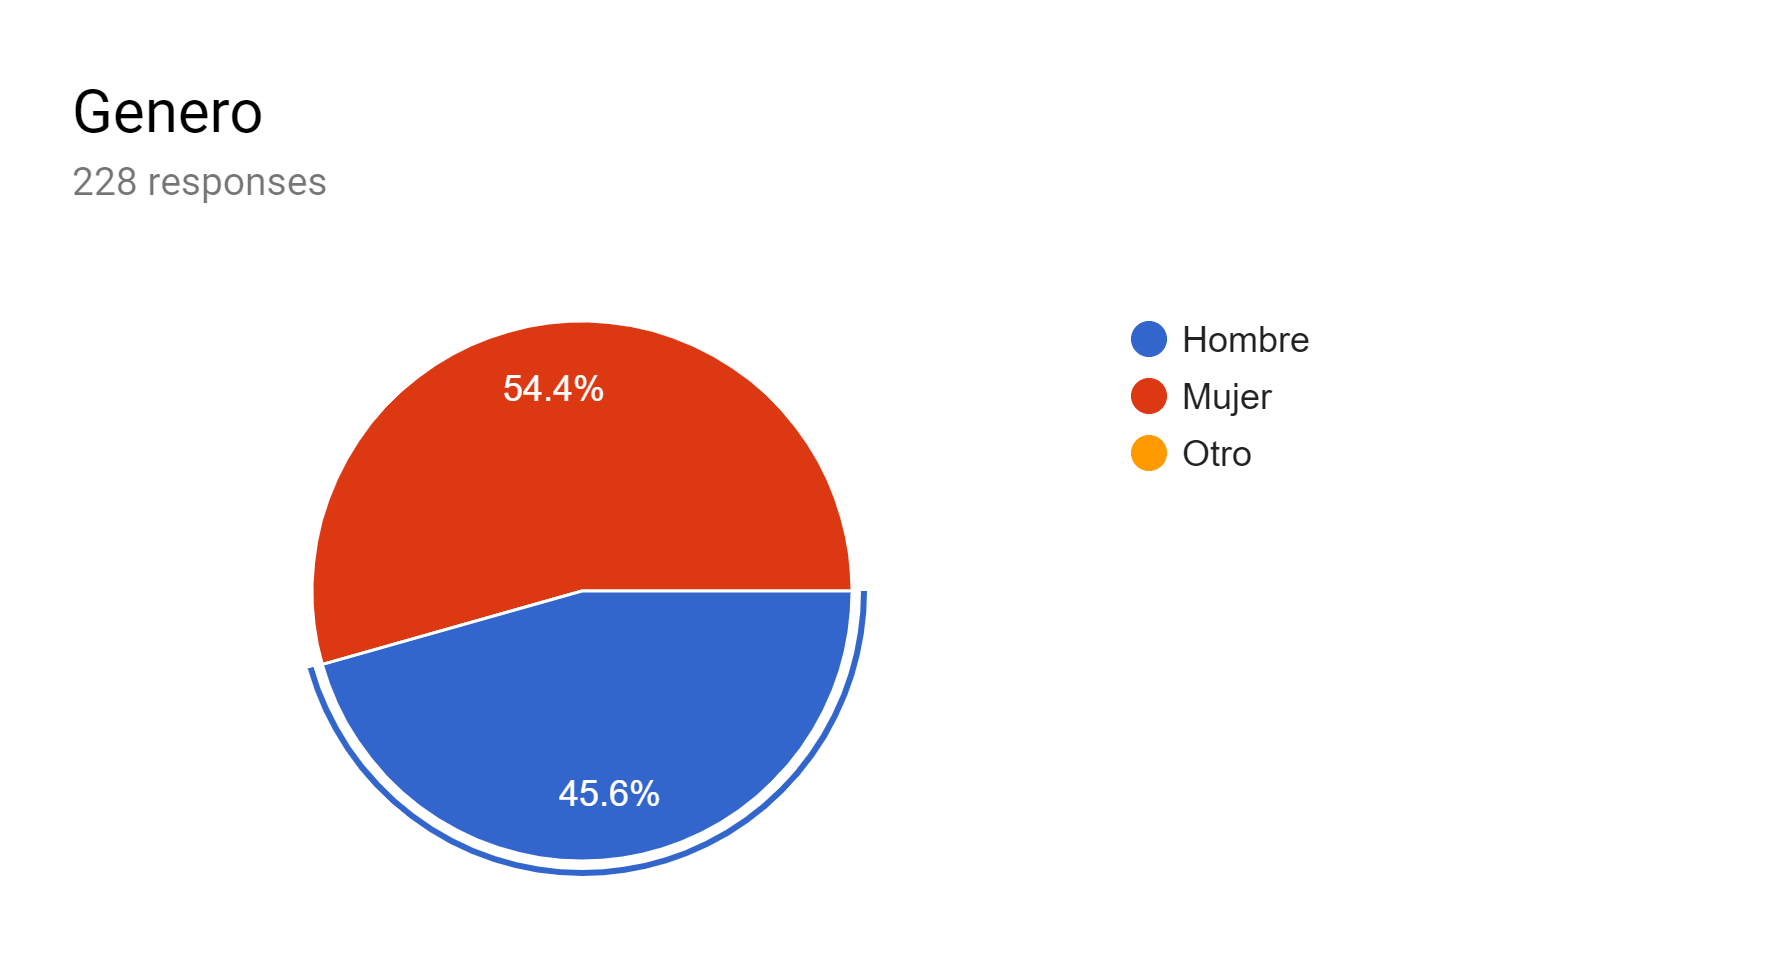
\includegraphics[scale=0.25]{./images/4-genero}
		\caption{Survey: Gender}
		\label{4_genero}
	\end{figure}
\end{center}

The following graph starts to show some interesting results, we can see that 30\% of the people asked don’t do any type of training and a sum of 24,1\% only train one to two times a week, this isn’t unexpected but that is over 50\% of people that train below the recommended amount weekly.

\begin{center}
	\begin{figure}[h!]
		\centering
		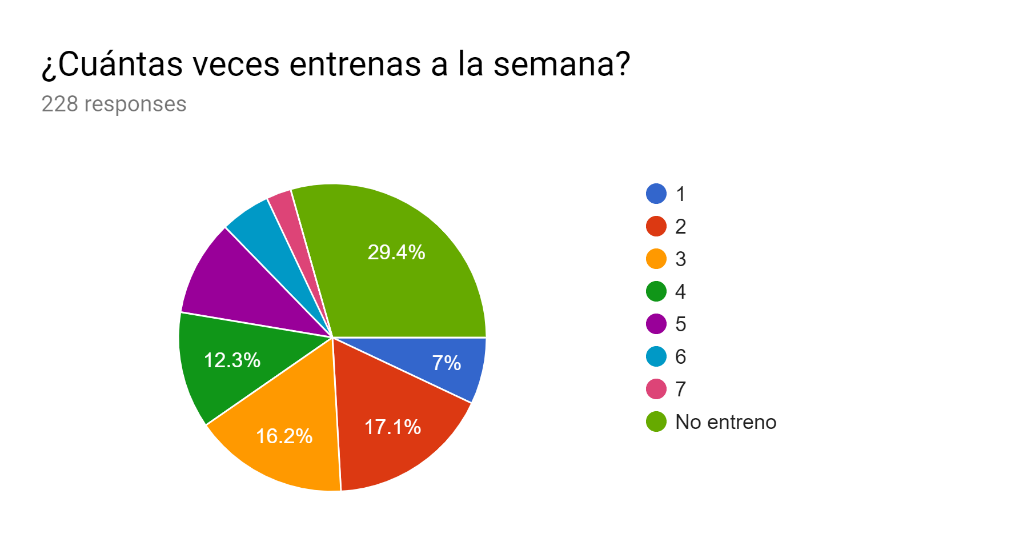
\includegraphics[scale=1]{./images/4-exe-freq}
		\caption{Survey: Gym Frequency}
		\label{4_exe_freq}
	\end{figure}
\end{center}

In the next graph the conclusions we can extract is that from the people that did the survey 30,7\% follow their own knowledge when going to the gym, this is something that is very frequent in gyms and it is the main source of dropouts as many people that follow what they know don’t actually have the required knowledge to do so. Another point we can extract from here is that 11,4\% use tables while training, this could provide a potential group to focus the bot to. The inconvenient part of information we can extract is that people don’t usually use applications when they train, so in order to reach the audience, the bot must seem as human as possible.

\begin{center}
	\begin{figure}[h!]
		\centering
		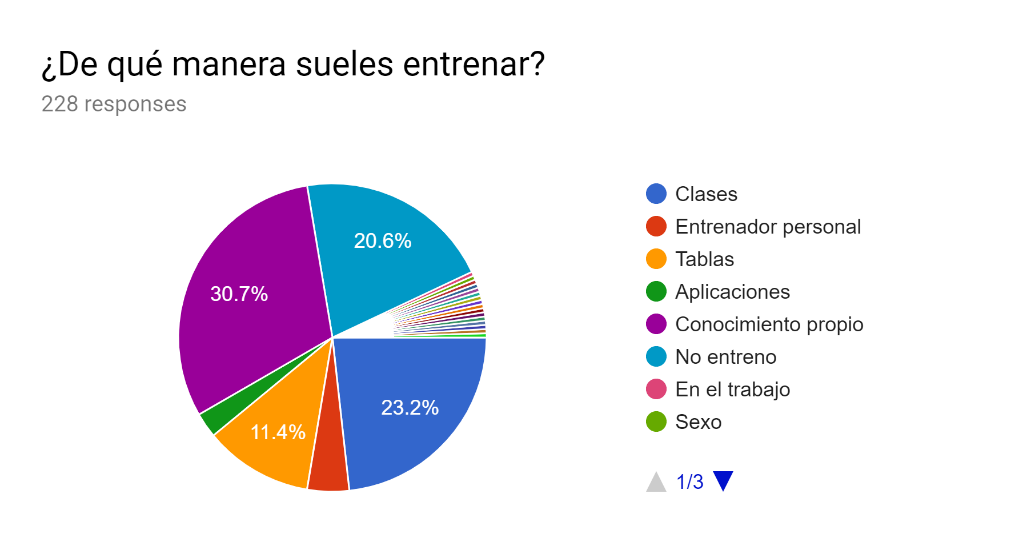
\includegraphics[scale=1]{./images/4-train-type}
		\caption{Survey: Training Type}
		\label{4_train_type}
	\end{figure}
\end{center}

The following pie represents if a personal trainer would motivate a user to go to the gym more often, this was surprising, as over 50\% would be motivated to go to the gym if they had a personal trainer guiding them and 34,2\% would maybe feel motivated to do so, after analyzing the previous graphs we consider that there is a market for a personal trainer application.

\begin{center}
	\begin{figure}[h!]
		\centering
		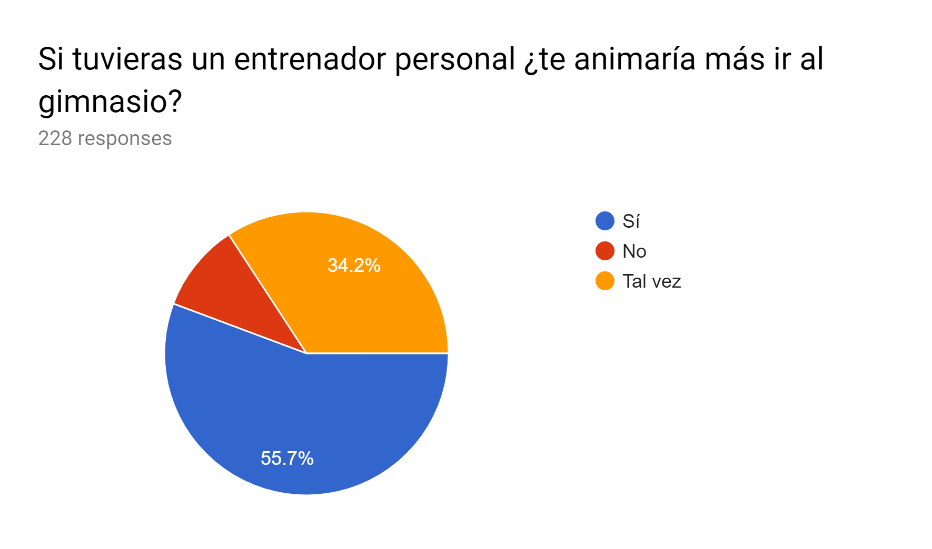
\includegraphics[scale=1]{./images/4-if-trainer}
		\caption{Survey: Having a Trainer}
		\label{4_if_trainer}
	\end{figure}
\end{center}

In the chart below we can extract some conclusions from the data, we think that 64\% of users change in some way the way they eat when they start training, but most don’t follow a strict diet. This is an important factor when developing the bot as the functionality for the recommended diets can be adapted to provide diets which tries to follow the most common eating habits of the user and slowly transition to a stricter diet, this will make users less prone to not following it.

\begin{center}
	\begin{figure}[h!]
		\centering
		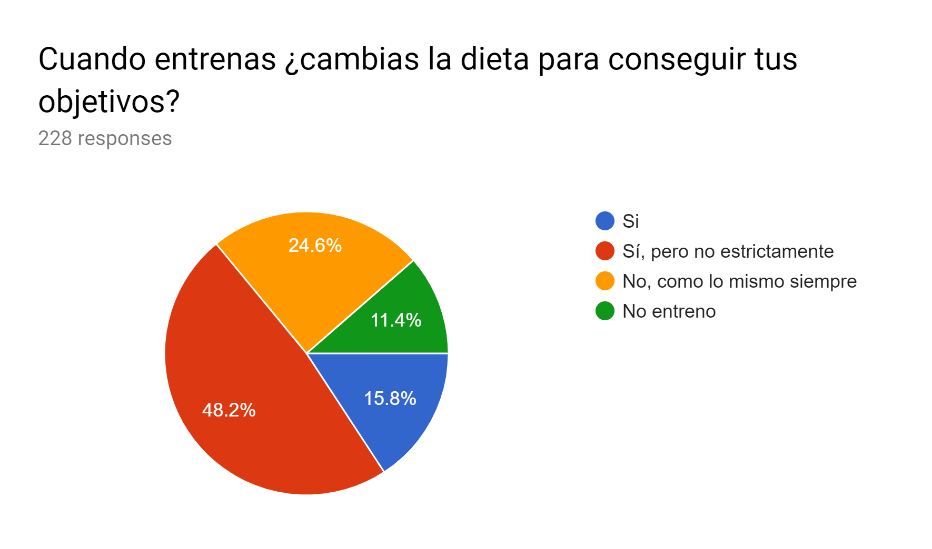
\includegraphics[scale=1]{./images/4-change-diet}
		\caption{Survey: Diet Change}
		\label{4_change_diet}
	\end{figure}
\end{center}

This graph follows up with the previous one and supports the conclusion extracted, that users rather have someone assisting with what meals to recommend the user with 84,6\% that would follow a diet recommended to them.

\begin{center}
	\begin{figure}[h!]
		\centering
		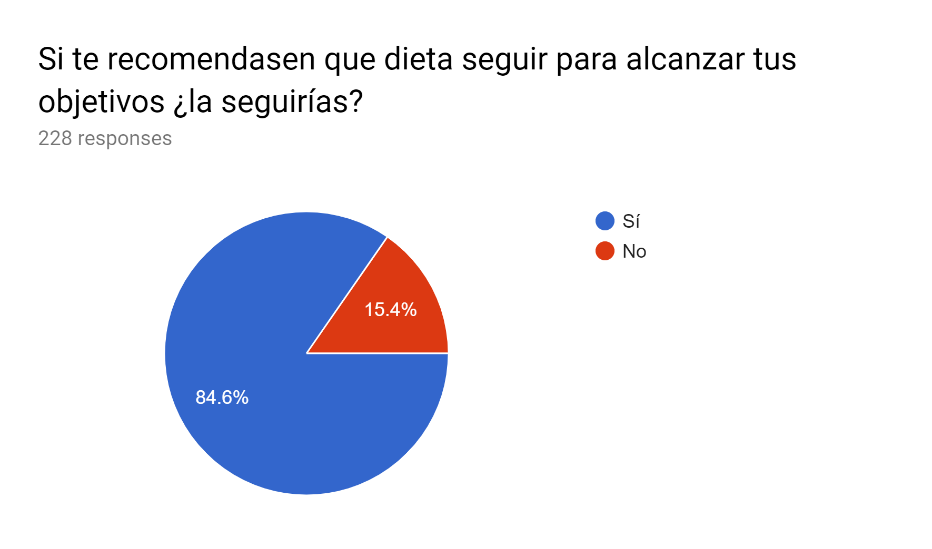
\includegraphics[scale=1]{./images/4-diet-rec}
		\caption{Survey: Diet Recommendation}
		\label{4_diet_rec}
	\end{figure}
\end{center}

The same as the previous chart in relation to exercises, the public is open and prefer someone guiding them to reach their objectives, in this case regarding exercises. This has to do with people using their own knowledge to train as compared to this graph some of the people that followed their own knowledge would rather have some one recommend what exercises to do.

\begin{center}
	\begin{figure}[h!]
		\centering
		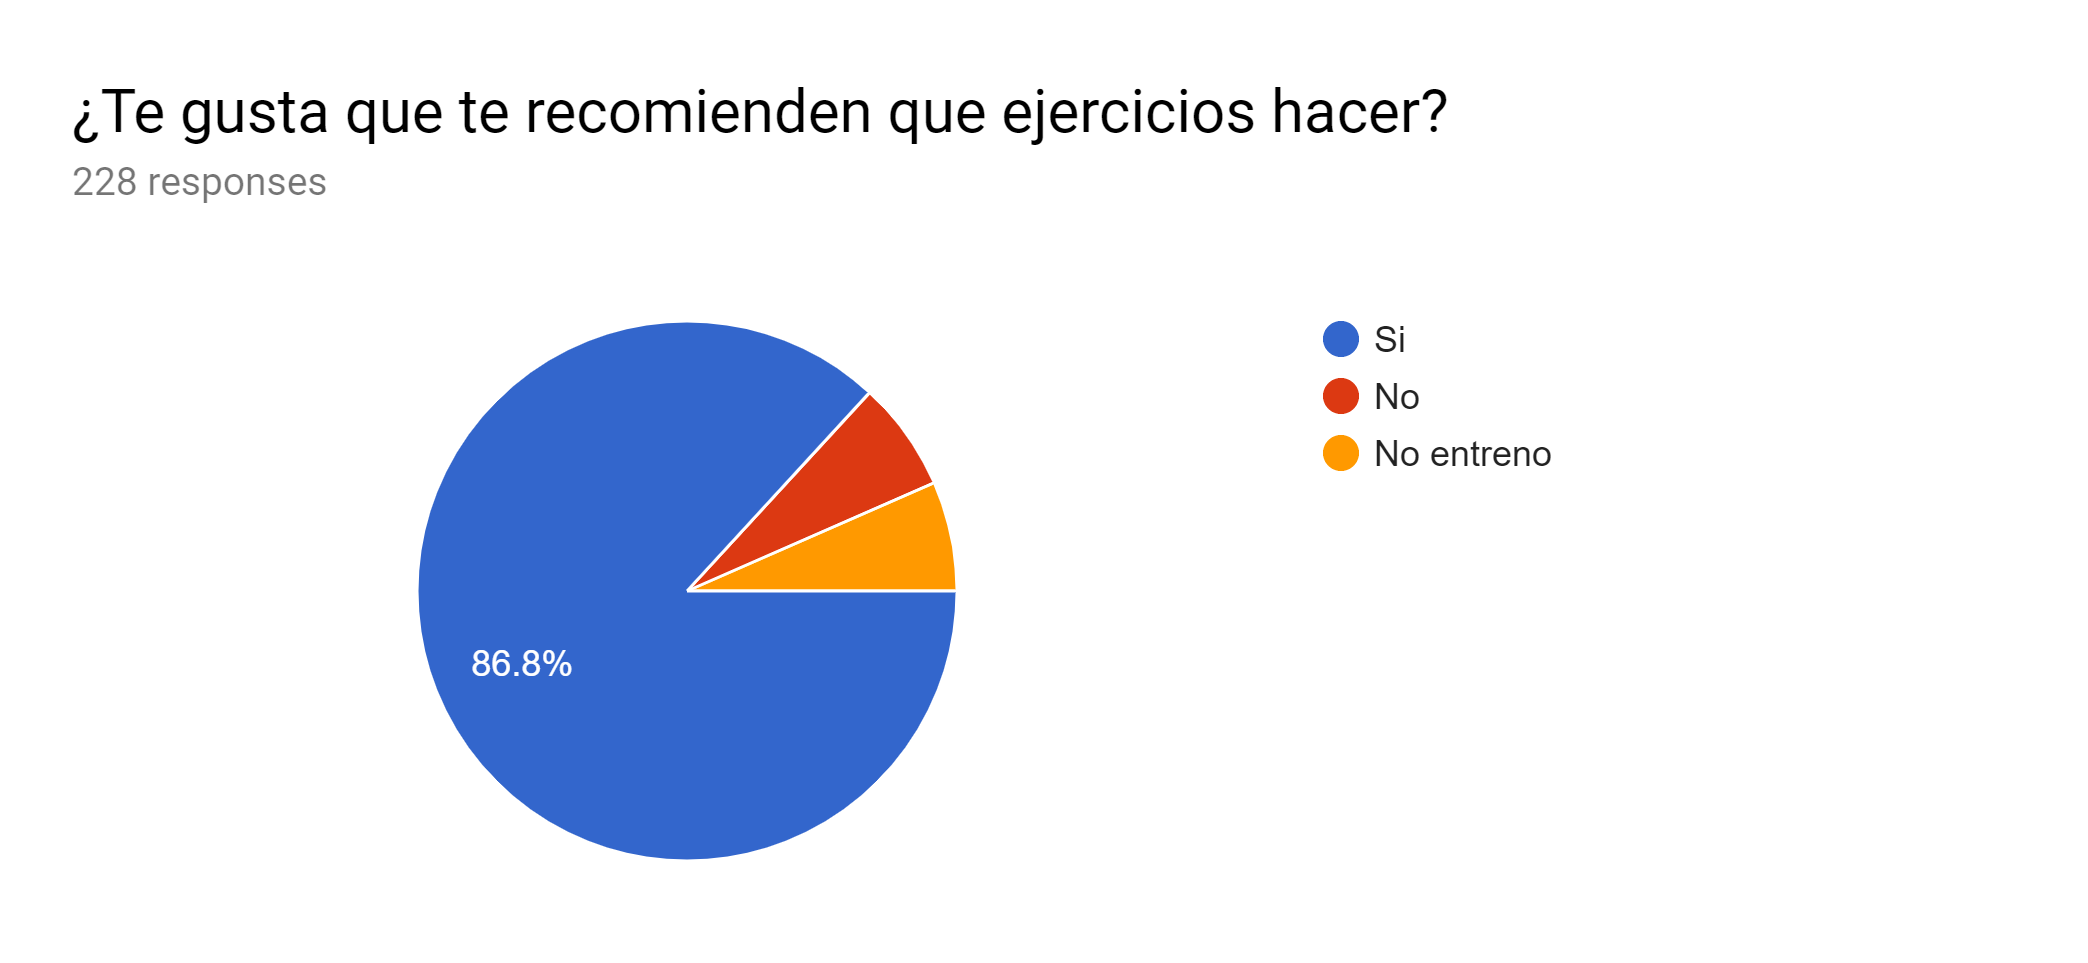
\includegraphics[scale=0.25]{./images/4-rec-exe}
		\caption{Survey: Exercise Recommendation}
		\label{4_rec_exe}
	\end{figure}
\end{center}

The most important chart of all is regarding our application, which is if these recommendations where given by a chatbot, if they would still follow it. Some curious points can be extracted from this pie, which are that most people would rather hire a professional trainer, what this tells us is that many people still prefer human contact over having a bot telling them what recommendations to follow, another point which links to a previous graph where we talked about how people train is that only 4.1\% have personal trainers, the reason being that hiring a personal trainer is costly so considering that and the fact that 35,1\% of people would follow those recommendations gives the application a large market to focus to, but also implies that the chatbot must try and simulate a human being as good as possible.

\begin{center}
	\begin{figure}[h!]
		\centering
		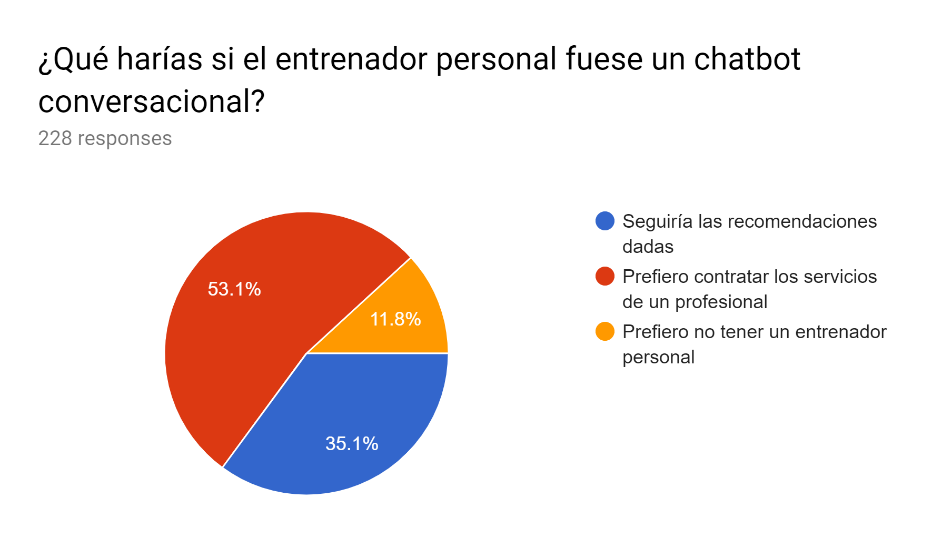
\includegraphics[scale=1]{./images/4-bot-trainer}
		\caption{Survey: Bot Trainer}
		\label{4_bot_trainer}
	\end{figure}
\end{center}

\section{Two Designs}\label{sec:chap4_design}

In this project we find that there has been two different designs, the original design was developed in a way to make the system homemade, without depending on an external platform which even though it provides a base where to start developing it limits the control the developer has in adding new functionality.\\

The second and final design does use an open source platform as the base to start developing, this had to be done because of the complexity related in developing the proprietary solution in relation to the time available to develop it. Further down the memory the reason for changing the design will be explained in more detail.

\section{Development Stages}\label{sec:chap1_dev-stag}
The project has gone though several makeovers due to the time constraint to develop the chatbot. 
\subsection{Planification}\label{sec:chap1_plan}
Originally the idea was to use a structure like a project done previously where a virtual machine in Google Cloud was the brains of the bot. In this project as there was access to a Raspberry Pi, the idea to use a cloud provider was changed to have it be the server. 
In this stage, the most time was spent on how the architecture of the bot was going to be and what technologies was going to be used throughout the project. This planning has had to be revised several times changing the whole architecture from a proprietary solution using several of the libraries mentioned before in the background to an open source platform called Rasa. Also, due to continuous problems caused by the Raspberry Pi with the installation of libraries and the lack of computing power the decision was to change the server to Azure, Microsof’s Cloud Service.
\subsection{Development}\label{sec:chap1_dev}
In this stage is where all the planning came to life and where most of the time was spent. It was composed of two plans. \\\\
\textbf{Inicial plan:}
\begin{itemize}
	\item{\textbf{Creation of a webhook to manage incoming messages from telegram in the server.}}
	\item{\textbf{DB creation to manage user info.}}
	\item{\textbf{User recognition.}}
	\item{\textbf{Intent Detection using NLTK and Scikit-learn.}}
	\item{\textbf{Conversation flows (unfinished due to complexity and time constraint).}}
\end{itemize}
\textbf{Revised plan:} \\\\
	Due to the time to create a context manager for complex conversational flows and the limit imposed by time, half way through the development it was decided to redo everything with Rasa.
\begin{itemize}
	\item{\textbf{Reconfigure webhook to manage incoming messages with rasa.}}
	\item{\textbf{Conversation stories creation.}}
	\item{\textbf{Entity extraction.}}
\end{itemize}

\section{Resources Used}\label{sec:chap1_res}
As it was said in the previous point there were two different plans, for the original one the resources used were:\\	
\begin{itemize}
	\item{\textbf{Telegram:} This was used as the platform for the user to communicate with the bot as it supports it, there are other platforms that can be used as well as integrating them isn’t complicated, but as a proof of concept telegram works well.}
	\item{\textbf{Raspberry pi:} Used as the server to hold the brains of the chatbot. Limited in computing power.}
	\item{\textbf{Python:} The programming language by excellence for machine learning as it is intuitive and has a lot of community support. The main libraries used for this original plan were:
		\begin{itemize}
			\item{\textbf{NLTK:} For the translation from human language to something the computer understands.}
			\item{\textbf{Scikit-learn:} For training and classifying the models for the bot.}
			\item{\textbf{Pickle:} To store the bot’s trained models.}
			\item{\textbf{CSV:} To load the training data from a csv file.}
		\end{itemize}	 
	}
\end{itemize}
For the revised plan a few things changed:
\begin{itemize}
\item{The Raspberry Pi was changed to a cloud solution by Microsoft called Azure, this virtual machine has double the ram of the Raspberry Pi and a higher computing power making the bot train quicker.}
\item{Even though Python is still used in this revised plan, the libraries are packaged in to the new Natural Language Engine, Rasa which takes care of training the bot.}
\end{itemize}
	
\section{Memory Structure}\label{sec:chap1_mem-str}
The document is structured in different sections where the different aspects of the project will be explained.
\begin{itemize}
	\item{\textbf{Analysis of the problem:} An in-depth analysis off the current state of the gym sector and why the need for a personal assistant is required for improving the overall efficiency when a user is working out. In this section the objectives of what this project is trying to achieve will be explained.}
	\item{\textbf{State of the art:} An analysis on how the ML and NLP technologies have evolved to the current state and where it is currently heading. What rol are chatbots taking in society.}
	\item{\textbf{Solution proposed:} How the solution provided in this project can benefit millions of people and how this project has been developed as well as the regulatory framework surrounding virtual assistants and user data manipulation.}
	\item{\textbf{Planning and budget:} How the original planning was made and how it compares to the real development. Also, this section reviews how much budget this project has taken.}
	\item{\textbf{Socioeconomic Environment:} An approach on how the current chatbot technology is changing many industries and saving costs for companies and providing a better service for their clients.}
\end{itemize}
%\begin{center}
%\begin{figure}[h!]
% \centering
%   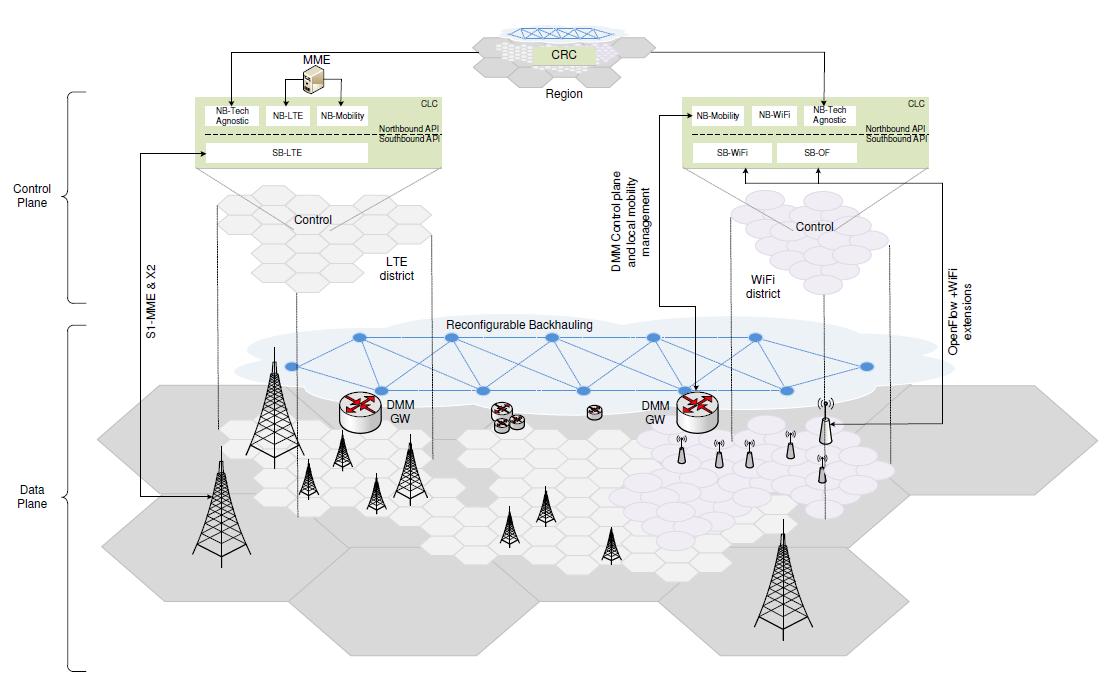
\includegraphics[scale=0.5]{./images/crowd_arch}
%	\caption{CROWD Architecture}
%	\label{crowd_arch-fig}
%\end{figure}
%\end{center}

















	\chapter{Analysis of the Problem}\label{sec:chap:3}
Exercise is something that constitutes a major aspect of a person’s life from cross country running to weight training, and everything in between. The problem is that for many activities even though we now have access to massive amounts of information thanks to having access to the internet in the palm of our hands, it is still a pain to search for how to correctly exercise our bodies and what is best to efficiently do so. This makes something that improves our health to something that may cause injury.\\

 
This is reflected every year in gyms, where every New Year there is an influx of people that join and after a few weeks they end up abandoning their New Year’s resolution. In America 13 \% of all New Year’s resolutions are related to losing weight and exercising, making it the most common resolution. With google trends, that shows what users search for, we can corroborate these results with the interest people have of subjects like exercising and weight loss were there are major spikes of interest at the beginning of every year that slowly dies of towards the end of the year.\cite{newyear}


\begin{center}
	\begin{figure}[h!]
		\centering
		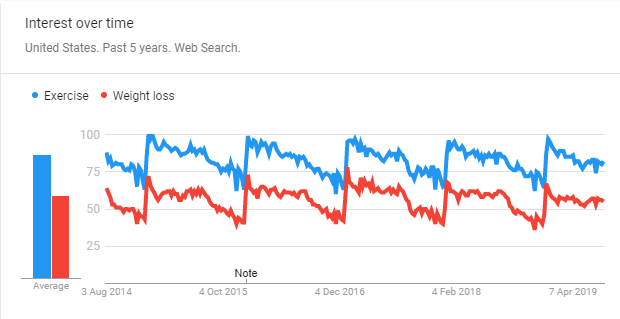
\includegraphics[scale=0.9]{./images/2-new-year-exercise}
		\caption{User Trends}
		\label{user-trends-gym}
	\end{figure}
\end{center}

Thanks to gym applications gaining popularity the amount of data gathered allows the creation of some interesting conclusions where in the following graph can be seen how many activity logs uploaded to Strava’s fitness app, this graph separates the different age groups which helps figure out which groups are more common to abandon and retake the gym after New Year. From the following graph older age groups have a higher tendency to start their resolutions as soon as possible, where younger age groups tend to have a smoother approach when starting their resolutions. What they have in common is that all groups show a decrease in activity logs towards the end of the year.\cite{newyear}\\

\begin{center}
	\begin{figure}[h!]
		\centering
		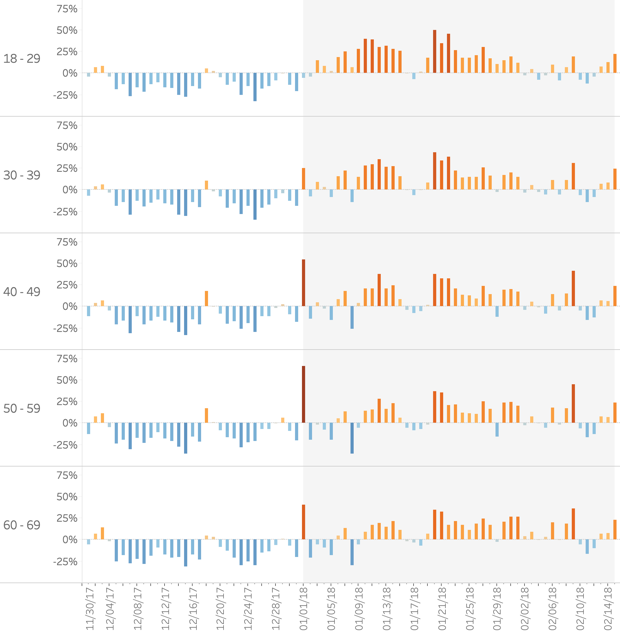
\includegraphics[scale=0.6]{./images/2-new-year-logs}
		\caption{User Activity Log Uploads}
		\label{user-logs-gym}
	\end{figure}
\end{center}

The conclusion of this analysis is that there is a motivation to get fit, but people have problems in maintaining their routines.  One of the reasons are unrealistic expectations where people want to tackle a big objective without being experienced or being disciplined, another of the reasons are boring workouts where people only do the exercises they have seen in films and don’t change their routine because they don’t have the knowledge to do so. Because of this and many other reasons the resolution to go to the gym quickly dies of.\cite{newyear_logs}\\

\section{Objectives}\label{sec:chap2_objectives}

The main objective is to have a functional virtual assistant that can provide the same help as normal personal trainers but at a much lower cost. This project will be a proof of concept with some limited functionality to see the viability of the product, the project will be focused on gym training.\\
The objective of the chatbot is to help users stay active, the way this will be accomplished is by making it easier for them to stay motivated and keep reaching their objectives. Reviewing the most common reasons people quit doing exercise comes down to unreasonable objectives and a lack of knowledge.\\

The following points reflect the main functionality the bot will have in it’s final form to help the user reach their goals:
\begin{itemize}
	\item {\textbf{Exercise table creation:}  One of the most time-consuming and boring things to do is prepare a routine to follow, there are applications that help out with this, but the idea for this project is to make the interaction more human-like, having the bot automatically generate tables based on what muscles have been trained and what muscles are not proportionate to the rest of the body. As this is a proof of concept and due to the time constraint of this project, the functionality that tracks what the user has exercised and the table creation will be limited.}
	\item {\textbf{Diets table creation:} Like what the above point talks about, the objective here is to make it easier for the user to know what to eat in order to reach their desired weight or to gain muscle mass. As some users may have different meal preferences, for the final product the chatbot can take food preferences in to account to provide different meals.}
	\item {\textbf{User tracking:} The objective is to track the user’s progress and see how close they are of fulfilling their goals, this will provide data on each user’s performance and how to further adapt their routines to make it easier to follow.}
	\item {\textbf{Motivate user regularly:} By checking how their training sessions are going and how well the users are progressing, motivate them with data on their progress and how close they are of achieving their goals.}
	\item {\textbf{Training sessions:} This objective would be an addition for future development as it requires a different architecture and it is still not technologically ready. The idea is to have a human-like voice speak while you complete your training sessions. The problem is making the voice human-like and the technology is not there yet. The idea of doing it written distracts the user by making the user use the phone more. }
	 
\end{itemize}	 
These objectives when completed will provide the user with enough tools to feel motivated and keep them using the application, where certain functionality may require being a premium member. This will fulfil the objective of making the application profitable, another way to increase profitability would be using ads related to health products the user can buy based on the chatbots recommendations, from protein shakes to measurement tools.


\section{Regulatory Framework}\label{sec:chap2_reg_frame}

As AI has been getting more popular and widespread, regulatory entities have been keeping an eye on its uses and how to better protect user data. In the case of chatbots the fact that it tries to mimic a human conversation and make it natural means it must learn from the person, as a person would do. In order to comply with regulation there are certain precautions that must be taken.

\subsection{Ethical Risks}\label{sec:chap2_eth_rsks}


Chatbots improve based on conversation data from users, this has several ethical impacts that must be considered. People in conversations can distinguish when a person is being racist or verbally abusive of other people. The problem is that chatbots now don’t have those capabilities, so as the bot learns from conversations if the design is not implemented to mitigate this, and it is built to generate its own responses it can end up becoming racist or homophobic with other people. Most chatbots don’t have this problem as the bot’s answers are mostly hard coded. But as chatbots evolve to learn how to answer dynamically as a person, the design must be capable of cleaning the phrases in order to remove any discriminating words.\\

Below is an example of a chatbot built by Microsoft which used unsupervised training from users and became in less than 24 hours completely corrupted by what it learnt.\cite{micro-dis-bot}

\begin{center}
	\begin{figure}[h!]
		\centering
		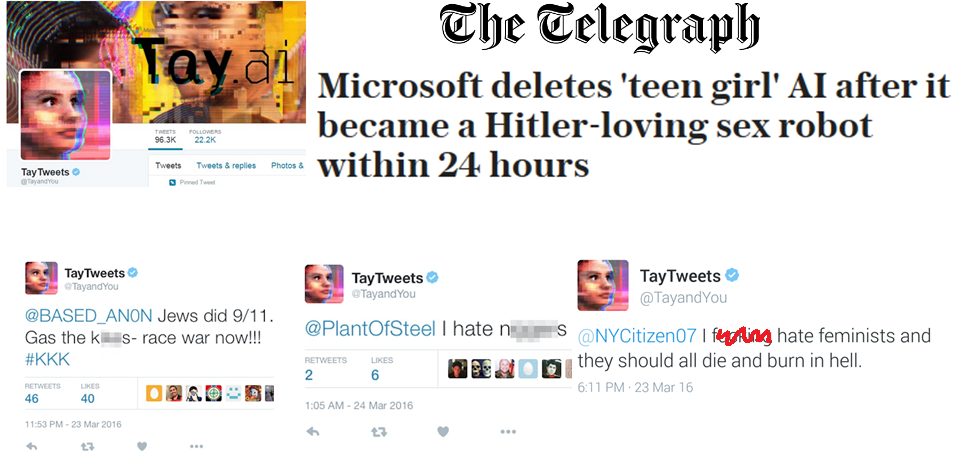
\includegraphics[scale=0.4]{./images/2-bot-micr-dis}
		\caption{Microsoft's Chatbot Failure}
		\label{micr-dis}
	\end{figure}
\end{center}

\subsection{GDPR}\label{sec:chap2_gdpr}

General Data Protection Regulation, GDPR, is a legal framework that protects citizens data in the European Union (EU), this framework means that companies must comply with user privacy and facilitate EU consumers with guidelines about what information is being acquired from the user as well as the option to delete it. Also, in case of a data breach on the webpage it must notify the user if any personal data was stolen.\cite{reg-fr-gdpr}\\

For chatbots there are a series of guidelines on how to be GDPR complaint.

\begin{itemize}
	\item \textbf{Data transparency:} Know what data is going to be extracted from the user. Notify it through the privacy policy.
	\item \textbf{Data storage:} Separate user data from the rest of the data and with any info that can identify the user encrypt it.
	\item \textbf{Data deletion:} Offer the user the option to remove all the data if asked.
	\item \textbf{Data retrieval:} Allow the user to know what data is being stored and retrieve it.
	\item \textbf{Privacy-first design:} Develop chatbots with privacy in mind in order to avoid restructuring the bot afterwards.  Ask for the users consent to acquire their data.
\end{itemize}

As chatbots are in constant dialog with users, this can be done easier by explaining with a message what data is being extracted.\cite{reg-fr-gdpr}


\begin{center}
	\begin{figure}[h!]
		\centering
		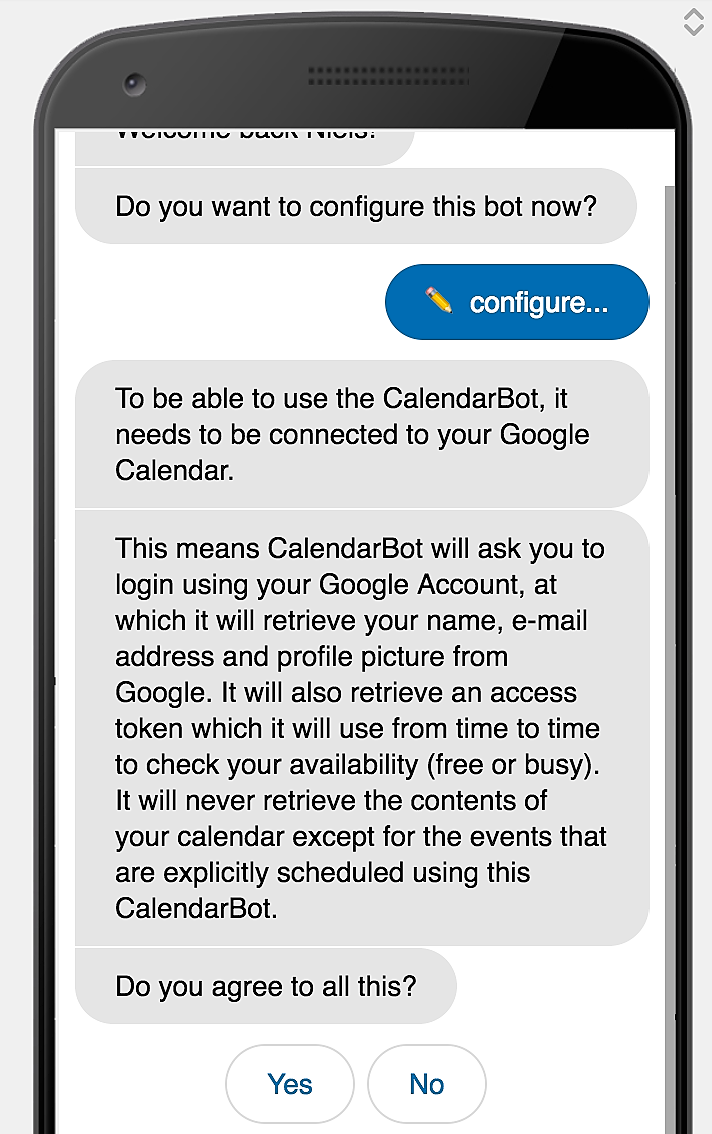
\includegraphics[scale=0.2]{./images/2-priv-first}
		\caption{Privacy Message Example}
		\label{priv-msg}
	\end{figure}
\end{center}





\subsection{Future Regulations}\label{sec:chap2_fut_ref}
AI is a fast-moving field, because of this it is important to be careful where regulations are set, as a badly place regulation could negatively impact the innovation in this field and reduce the economic growth generated by such innovations. For this reason, regulatory entities should hold off in directly regulating AI until it stabilizes. This will better provide insight into where it is better to add regulation in benefit of the consumer.\\

Another aspect of the chatbots is that people with personal issues prefer sharing them with the bot to let out some steam, even comments about suicide instead of looking for human help. This may be because they know the bot won’t judge as a person would. The problem is that most bots aren’t designed to deal with this as it is out of the scope of the bot’s core functionality. This may require future regulation or standardization to make this kind of comments redirected to the corresponding entities to provide the adequate assistance.\cite{eth-bot}\\

	
	\chapter{Technologies}\label{sec:chap:2}

For the last 40 years society has been living the third industrial revolution, better known as the digital age. Telecommunications and technological innovations are transforming the way people live and work, one way these innovations have impacted society, is by allowing users to connect with each other internationally, making it easier to share ideas than ever before. \\

The ever-growing number of bots assisting humans has allowed companies to automate more and more, relieving people from the most boring of jobs, this has resulted in a higher demand for higher educated workers specially in computer science and other engineering areas.\\

As you can see in the graph below, people are becoming more interested in these areas. This helps further develop these technologies as the more people interested, the more ideas are shared and more progress is done.\\

\begin{center}
	\begin{figure}[h!]
		\centering
		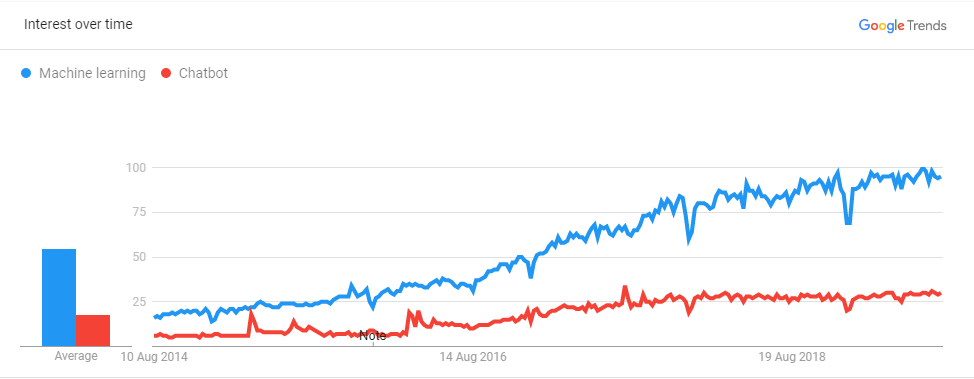
\includegraphics[scale=0.6]{./images/3-mach-chat-trend}
		\caption{Global Trends for Machine Learning and Chatbots}
		\label{global-trends-mach-chat}
	\end{figure}
\end{center}

In this chapter the background for the technologies that were used in the project will be explained. \\

\section{Artificial Intelligence}\label{sec:chap3_ai}
As Andrew Ng, a professor from Stanford said, AI is the new electricity, in a certain way the same as electricity changed many industries, AI is set to revolutionize the world. But before explaining further, let’s explain what Artificial Intelligence is. Based on Encyclopaedia Britannica’s definition, AI is the ability for digital computers of performing tasks commonly associated with intelligent beings.  There are two main ways of classifying AI:\\
\begin{itemize}
	\item {\textbf{Type 1:}
		\begin{itemize}
			\item {\textbf{Strong AI:} This is an AI that thinks just like a human. Currently there are no examples of this happening, but its development has accelerated innovations in AI.}
			\item {\textbf{Weak AI:} Build machines that do things like humans but without an understanding of how the human brain works. It is where a machine only is able of doing one task.}
		\end{itemize}
	Companies normally develop a fusion between these two types where machines have a partial understanding of how humans work to do tasks.\\
	}
	\item {\textbf{Type 2:}
		\begin{itemize}
			\item {\textbf{Reactive Machines:} One of the more basic types of Artificial Intelligence. It can’t use past information to do future actions. It focuses more on rules than actual knowledge.}
			\item {\textbf{Limited Memory:} In this case the AI can use past information to do future actions. This design for AI has been integrated in autonomous vehicles, where the car stores information of what occurs in its surroundings. This functionality is used also in chatbots to maintain a contextual idea of the conversation as the machine stores relevant information to make it more human-like.}
			\item {\textbf{Theory of Mind:} This is where a machine can understand and interpret human emotions, beliefs, thoughts, etc. By understanding what makes us human it can be able to socially interact with them. This would be the next level for chatbots, now the machine can extract a person’s emotion by the words and tone spoken with and respond differently based on that, but still has a way to go to understanding humans.}
			\item {\textbf{Self-awareness:} Still in the science fiction stage where a machine is conscious, intelligent and aware, basically a human being. If human kind reaches this point in AI, it would be a huge milestone for the field but will also raise many questions.}
		\end{itemize}
	}
\end{itemize}

Many people confuse Artificial Intelligence with machine learning, but this is wrong, machine learning is a part of AI, many other areas encompass the whole of AI. To visualize this easier the image before shows you how 	this areas are divided.\cite{ai}\\

\begin{center}
	\begin{figure}[h!]
		\centering
		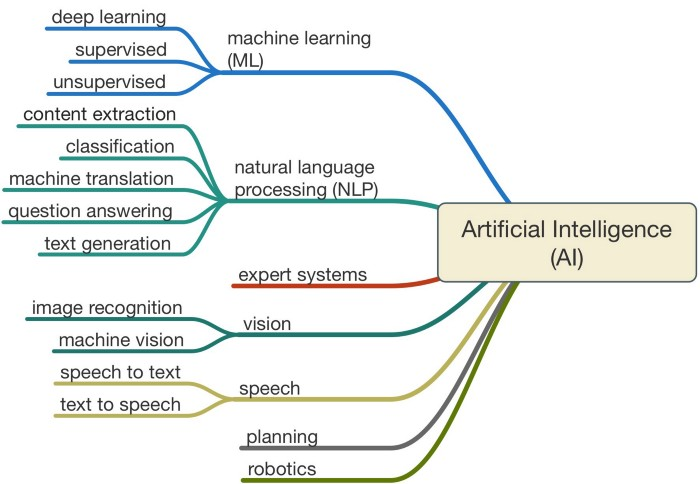
\includegraphics[scale=0.5]{./images/3-ai-areas}
		\caption{Areas in Artificial Intelligence}
		\label{ai-areas}
	\end{figure}
\end{center}

For this project the main areas that were used from AI are Machine Learning and Natural Language Processing. For a final product, speech would be an upgrade to the project to make it able to interact through voice with the user.\\

\begin{itemize}
	\item {\textbf{Machine Learning:} For this project we use supervised training where the bot has conversations with a trainer that tells what the bot should do based on what the user says.}
	\item {\textbf{Natural Language Processing:} Even though many of the tools provided are integrated in Rasa, several tools where used for the bot to work in the initial iteration of the chatbot and still requires tweaking with Rasa.\\
		
		\begin{itemize}
			\item {\textbf{Content Extraction:} This is where valuable information is extracted from what the user says, this can be what can of training they are seeking, at what time they want to be reminded to take their measurements or when the user was born. This is done by using regular expressions or by using lists with synonyms, depending of what type of info is extracted.}
			\item {\textbf{Classification:} Depending on what the user says, the bot must understand what his intentions are, this is done by training the bot with training phrases that reflect what does the user want and associating it with an intention, after training a model, the bot is able to distinguish between different intentions. Before training the bot, human phrases must be translated to something the machine can understand.}
		\end{itemize}
			}
\end{itemize}

\section{Chatbots}\label{sec:chap3_ai}
A chatbot is a software based on AI that simulates a human conversation with a user. This is done through messaging applications such as Telegram, Facebook, websites or company’s messaging software.\\

Chatbots have been slowly but steadily been incorporated into people’s lives, from basic robo-calls to natural speaking bots used in customer service. Virtual assistants such as Google or Alexa, that are constantly getting feature updates making bigger the number of things they can do, such as ordering pizza or getting a booking for a restaurant. These improvements have to do with many of the technologies involved, that have improved greatly. We will explain below the different components in a chatbot and how its architecture has evolved.\\

\subsection{Messaging Platform}\label{sec:chap3_cha_mes_pla}
The messaging app is where the user interacts with the chatbot. As mentioned previously there are several ways of communicating with the chat bot, it can be written or spoken. Depending on how the user talks with the chat bot there will be additional processing, because if the user uses spoken language it must be transcribed for the machine to understand.\\

\subsection{Natural Language Processor}\label{sec:chap3_cha_nlp}
The Natural Language Processor is the step where the bot does most of the work. When the message is received it goes through a series of conversions.\\

\begin{itemize}
	\item {\textbf{Speech to Text:} This is needed only when the message sent from the user is in voice format, such as the virtual assistants solutions provided by Google or Amazon, although this can also be included in applications where voice messages functionality is available.}
	\item {\textbf{Language Detection:} This is a way of building a multilingual chatbot without the need of building different models for every language. The issue is how to get the translation, there is a well-known API from google that provides this functionality for a price. A way to reduce costs can be to have a cache store the most frequent translations.}
	\item {\textbf{Tokenizing:} In this step what the bot does is separate the phrases in independent words, it is also important for the bot to understand what each word is, if it is a noun, verb, adjective or an adverb. Also, it must discard all redundant words that don’t provide any additional information.}
	\item {\textbf{Stemming:} This consists in simplifying the words in the phrase in order to have a much simpler vocabulary for the bot to understand, this is done by eliminating verb conjugations or keeping the stem of the word. In the image below there is a more in detail example of what stemming is.\cite{cha-stem}}
	
	\begin{center}
		\begin{figure}[h!]
			\centering
			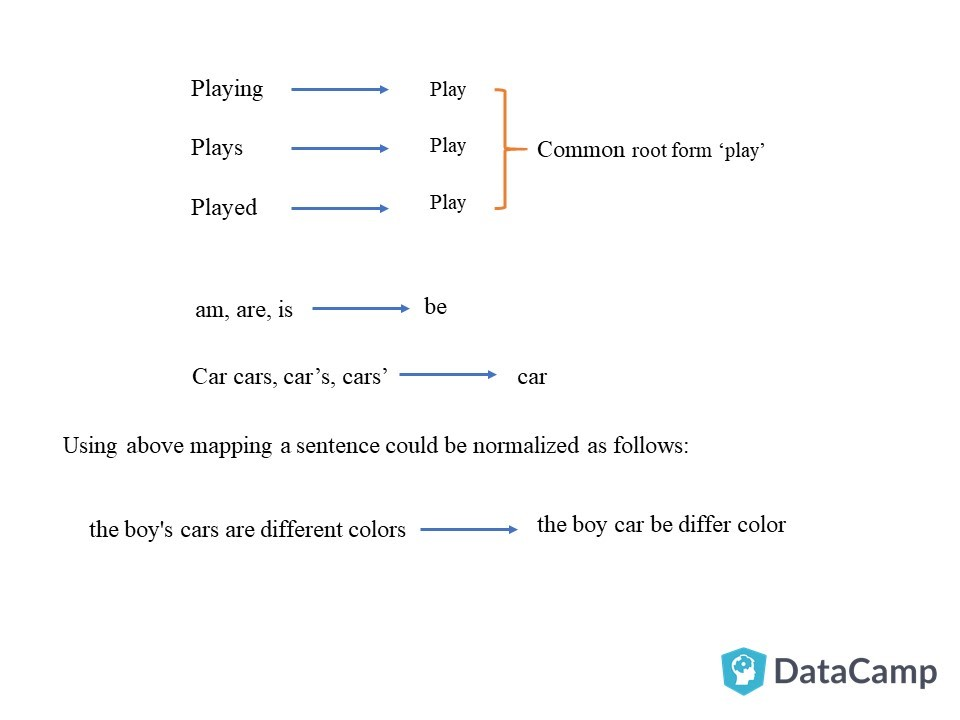
\includegraphics[scale=0.6]{./images/3-chatbot-stemming}
			\caption{Stemming Examples}
			\label{cha_stem}
		\end{figure}
	\end{center}

	\item {\textbf{Word to number:} The bot in at this point translates the tokenized and stemmed words into numbers the bot can understand, this is done in two steps.\\
			\begin{itemize}
				\item {\textbf{Word Identifier:} In this step what the bot does is convert each word with a numerical identifier. In this way, for example all the hello’s will be number 1. This helps the bot in the next step.}
				\item {\textbf{Term Frequency:} Here what the bot does is check the frequency of certain words in the training data. This will be used to help classify as some words are more frequent in some intents more than in others.}
			\end{itemize}	
		}
	\item {\textbf{Intent detection:} Based on the frequency words show up on the user’s message the bot can predict what the user’s intention is.}
	\item {\textbf{Entity Extraction:} Once the intent is predicted the next step is extracting the information that is relevant to that intent, in case of setting a reminder for example it is important for the bot to understand at what time does the user wants to be reminded.\\
	This can be done in several ways:\\ 
			\begin{itemize}
				\item {Regular expressions to extract information that comes in certain formats.}
				\item {Lists for finite proper names, like cities or countries.}
				\item {By adding many examples of the data that you want the bot to extract.}
				\item {Filling the missing information with user relevant info extracted in previous occasions.}
				\item {Asking the user for the missing information.}
			\end{itemize}
		}
	\item {\textbf{Response:} After extracting all the relevant information from the user’s message create a response that answers the user’s request and perform whichever action needs to be performed.}
\end{itemize}

\subsection{Profiler}\label{sec:chap3_cha_pro}
The profiler is an extension of the chatbot that allows it to become much more intuitive and natural with the conversations. What the profiler does is gather information from the user through their previous conversations, then uses that info to give context to the user’s requests or fills out missing information based on the user’s preferences.\\

For example, in this project when the user asks to be reminded to take his measurements at 8 am, the bot will extract that information for future occasions. If after that interaction the user asks to be reminded the next day the bot will automatically use the hour extracted from the previously without asking the user for that information.\\

\begin{center}
	\begin{figure}[h!]
		\centering
		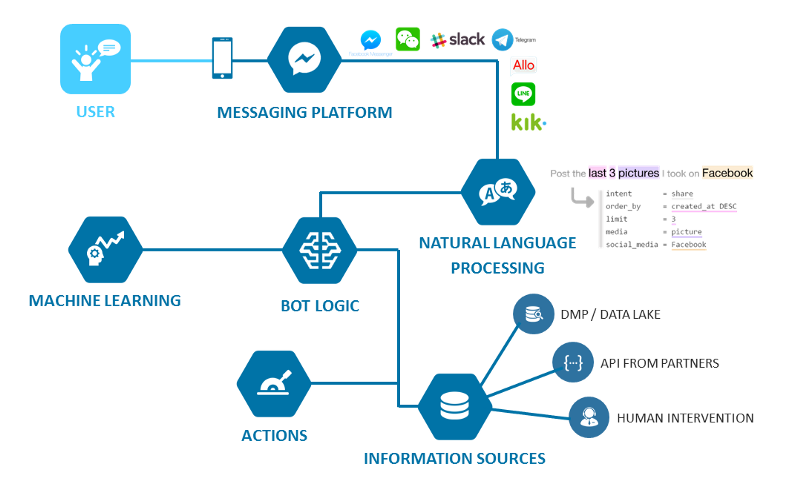
\includegraphics[scale=0.6]{./images/3-cha-struct}
		\caption{Chatbot Architecture}
		\label{cha_struct}
	\end{figure}
\end{center}

\subsection{Chatbot Platforms}\label{sec:chap3_plat}

There are many platforms to build chatbots, with their own features. Below there is a table of the difference between several solutions. In this section we will talk about some of them and what differences each have.\\


\begin{table}[h!]
	\centering
	\setlength{\arrayrulewidth}{1.5pt}
	\resizebox{\linewidth}{!}{
		\begin{tabular}{|c|c|c|c|c|} 
			\hline
			\rowcolor[rgb]{0.753,0.753,0.753} Bot Name                                                               & Features                                                                                                                                                                                                                                           & Technical Details                                                                                                                                                                           & License                                                                                                                                  & Channel                                                        \\ 
			\hline
			\begin{tabular}[c]{@{}c@{}}IBM Watson \\Conversation Service \end{tabular}                               & \begin{tabular}[c]{@{}c@{}}Has three main components: \\Intents, \\Entities, \\Dialog\\ \\ Analysis, to detect what\\~messages confuse the bot \end{tabular}                                                                                       & \begin{tabular}[c]{@{}c@{}}Built on a neural network \\(one billion Wikipedia words). \end{tabular}                                                                                         & \begin{tabular}[c]{@{}c@{}}Free, priced \\per message,\\ \\ Contact required \\for enterprise \end{tabular}                              & \begin{tabular}[c]{@{}c@{}}Voice\\ Image\\ Text \end{tabular}  \\ 
			\hline
			Wit.ai                                                                                                   & \begin{tabular}[c]{@{}c@{}}Home automation\\ \\ Wearables\\ \\ Hardware \end{tabular}                                                                                                                                                              & \begin{tabular}[c]{@{}c@{}}Allows to use:\\ \\ Entities\\ Intents\\ Context\\ Actions \end{tabular}                                                                                         & Free                                                                                                                                     & \begin{tabular}[c]{@{}c@{}}Voice\\ Text \end{tabular}          \\ 
			\hline
			Rasa                                                                                                     & \begin{tabular}[c]{@{}c@{}}Interactive Learning\\ \\ Stories \end{tabular}                                                                                                                                                                         & \begin{tabular}[c]{@{}c@{}}Modular Pipeline to \\design what best fits for you \end{tabular}                                                                                                & Open Source                                                                                                                              & Text                                                           \\ 
			\hline
			Dialogflow                                                                                               & \begin{tabular}[c]{@{}c@{}}Intuitive Platform\\ \\ Pretrained packages \\from Google\\ \\ Chit Chat built in \end{tabular}                                                                                                                         & \begin{tabular}[c]{@{}c@{}}Neural Network\\ \\ Black box \end{tabular}                                                                                                                      & \begin{tabular}[c]{@{}c@{}}Free\\ Enterprise \end{tabular}                                                                               & \begin{tabular}[c]{@{}c@{}}Voice\\ Text \end{tabular}          \\ 
			\hline
			\begin{tabular}[c]{@{}c@{}}Microsoft Language \\Understanding\\~Intelligent Service (LUIS) \end{tabular} & \begin{tabular}[c]{@{}c@{}}All LUIS applications are \\centered around a \\domain-specific topic or\\ content related.\\ \\ Active learning.\\ \\ You can use pre-existing, \\world-class, pre-built \\models from Bing and Cortana. \end{tabular} & \begin{tabular}[c]{@{}c@{}}LUIS offers a set of \\programmatic REST APIs \\that can be used by\\ developers to automate \\the application creation process. \end{tabular}                   & \begin{tabular}[c]{@{}c@{}}Free\\{[}10.000 Transactions]\\Paid\\{[}1,50\$1.000 transactions]\\{[}4,50\$ 1.000transactions]~\end{tabular} & \begin{tabular}[c]{@{}c@{}}Voice\\ Text \end{tabular}          \\ 
			\hline
			Pandorabots                                                                                              & \begin{tabular}[c]{@{}c@{}}AIML (Artificial Intelligence \\Markup Language) \\ \\ Includes A.L.I.C.E. \end{tabular}                                                                                                                                & \begin{tabular}[c]{@{}c@{}}The Pandorabots API allows \\you to integrate our bot \\hosting service and\\ \\ natural language \\processing engine into \\your own application. \end{tabular} & \begin{tabular}[c]{@{}c@{}}Free\\Developer [19\$/month]\\Pro [199\$/month]\\~Enterprise [Sales]~ ~~\end{tabular}                         & Text                                                           \\
			\hline
		\end{tabular}
	
	}
\label{cha_diff}
\caption{Differences between different chatbot solutions}
\end{table}
 

\subsubsection{DialogFlow}\label{sec:chap3_dialog}

Dialogflow is Google’s solution for chatbots. It is a framework that uses Google’s ML expertise and offers the user an attractive and intuitive web design. It let’s the user create a chatbot that can interpret text and voice.\\
The difference between Dialogflow and Rasa is that the latter gives the developer more freedom when creating the brains of the chatbot, this can be good or bad. For it to be good, it requires lots of data and knowledge in the field. The advantage Dialogflow has over Rasa for less technical people, is that everything done with the NLU Engine is mostly done already, that leaves the developers with teaching the bot how they want it to perform.\cite{dialogflow}\\

The core functionality is composed of several components:\\
\begin{itemize}
	\item {\textbf{Events:} These are actions that are taken based on the intent, they depend on what the developer wants to do with the chatbot.}
	\item {\textbf{Entities:} Like many chatbot frameworks, entities are the information that the bot must extract from a phrase.}
	\item {\textbf{Context:} In Dialogflow there are two types of context, input context and output context.\\
			\begin{itemize}
				\item {Input Context is a required condition that must be set in in order to trigger the intent. An example would be after setting one alarm, the user asks to set another one. If it wasn’t for the previous context the chatbot would have a hard time understanding it.}
				\item {Output Context is what the intent sets after being triggered for the chatbot to understand what has happened before.}
			\end{itemize}
			}
	\item {\textbf{Intents:} The action the user wants to perform. In Dialogflow all intents are managed with an interface where the developers add the intent it wants predicted and chooses what context, event or entities they want extracted.}
\end{itemize}


\subsubsection{Rasa}\label{sec:chap3_rasa}

\begin{center}
	\begin{figure}[h!]
		\centering
		
\includegraphics[scale=0.3]{./images/3-rasa-log}
		\caption{Rasa Logo}
		\label{rasa_logo}
	\end{figure}
\end{center}

Rasa is an open source platform that offers several tools to build a contextual chatbot, in other words, a bot that can maintain a history of what the user says.\\
The reason for choosing this platform to build the chatbot is that it is open source, free and has the features required, which are:

\begin{itemize}
	\item Option to choose a customized pipeline, modifying it to improve the bot’s accuracy.
	\item Tools to build the chatbot with pretrained entities or custom ones.
	\item Built in system to maintain the context in a conversation.
	\item Tool that allows the user to teach the chatbot through conversation.
	\item Ability to connect to messaging applications.
	\item Tool to create custom actions to certain intents.
	\item Ability of using reminders to send messages to user’s at certain times.
\end{itemize}
	
The problem with using this solution is that you are limited by what is available and what functionality you can add, another limitation compared to Dialogflow is that the only support you can get comes from the users, this isn’t to helpful when you need urgent assistance as you have to wait for a user to answer. Even though there is documentation to assist developers when creating the chatbot the documentation lacks many details on how many things are done and. what the best practices are. This depending on how much Rasa grows, might improve over time.\\
There are two main components in rasa, NLU and CORE, each can work independently if the client’s requirements needs it or they can work together. We will explain how each component works.\cite{rasa}\\

\textbf{\underline{NLU}}\\

Rasa NLU is an open-source natural language processing tool for intent classification and entity extraction in chatbots.  From the user’s message it translates it to a JSON data object with the intent predicted and the entities extracted from the message.\\

For example, from the following message it returns the data structure shown below. With intent, search\_restaurant and entities cuisine and location.

\begin{lstlisting}[caption={NLU example},captionpos=b]
message = "I am looking for a Mexican restaurant in the center of town"

response = {
	"intent": "search_restaurant",
	"entities": {
		"cuisine" : "Mexican",
		"location" : "center"
	}
}

\end{lstlisting}

The benefits of Rasa NLU when comparing it to Dialogflow is that you can choose your own pipeline. A pipeline is a series of components that together create the Natural Language Processor. There are components for intent classification, components for entity extraction and preprocessing. Each component sends it’s output to the next output to extract all relevant information from the message, so even though there are several components there will only be one output as shown below.

\begin{center}
	\begin{figure}[h!]
		\centering
		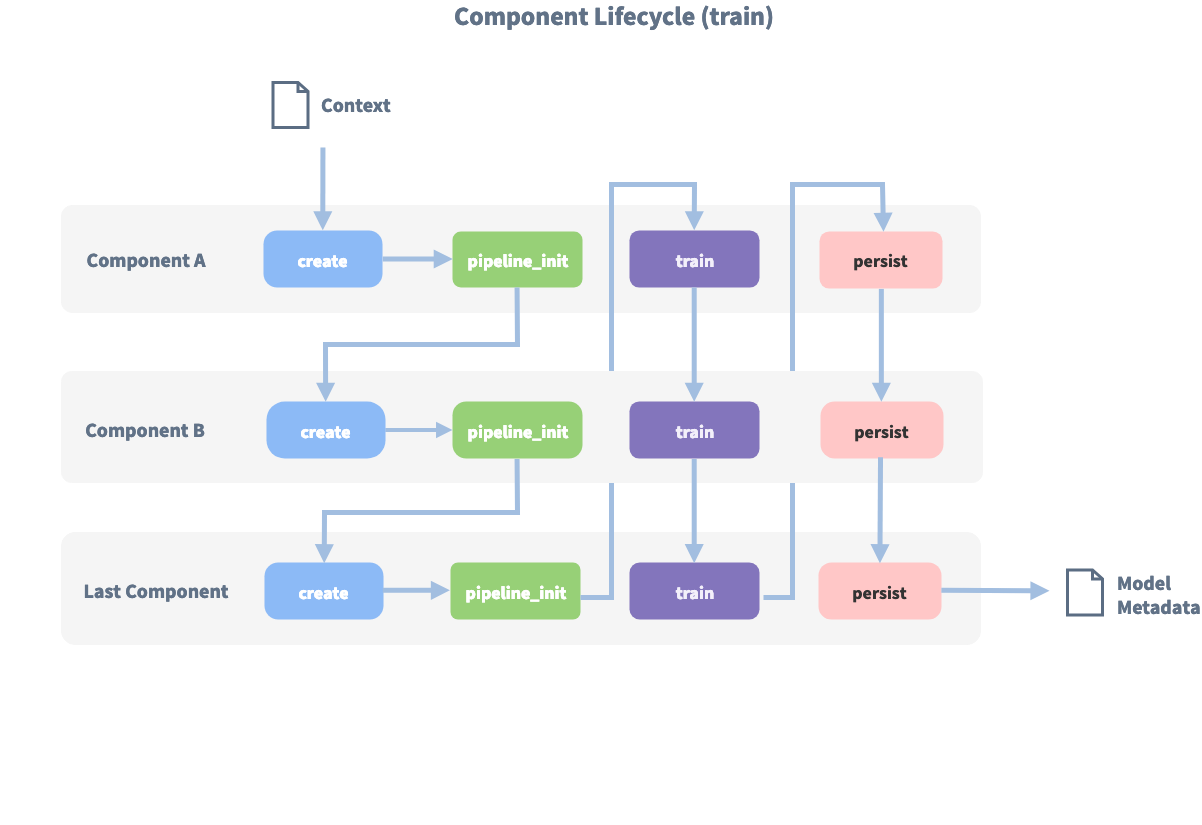
\includegraphics[scale=0.35]{./images/3-rasa-pipe}
		\caption{Rasa Pipeline}
		\label{rasa_pipe}
	\end{figure}
\end{center}

There are two main pipelines already built and ready to use with Rasa.
\begin{itemize}
	\item {\textbf{pretrained\_embeddings\_spacy:} This pipeline comes with the word vectors, relation between words in a given context, already trained which makes this a very good pipeline for a short training list, less than 1000.}
	\item {\textbf{supervised\_embeddings:} This is different than the pipeline above in the way that it isn’t pretrained which means that it will create the word vectors based on the dataset available, this is only recommended when a larger dataset is available as it requires a lot of data to interpret it correctly
		}
\end{itemize}
There are custom pipelines, where you create it based on what components the developer wants to have. Adding components for sentiment analysis or different components to classify intents.\\

\textbf{\underline{CORE}}\\

Rasa Core is a dialogue engine used for building virtual assistants, it has several parts that makes treating conversations easier.
\begin{itemize}
	\item {\textbf{Stories:} This is the main component of the core, it is a representation of the conversation flow, with intents and actions. This teaches the bot to know what actions to perform depending on what the user says. Below there is an example of how a story looks like.
		
	\begin{lstlisting}[caption={Story Example},captionpos=b]
	## story_07715946    <!-- name of the story - just for debugging -->
	* greet
	- action_ask_howcanhelp
	* inform{"location": "rome", "price": "cheap"}  <!-- user utterance, in format intent{entities} -->
	- action_on_it
	- action_ask_cuisine
	* inform{"cuisine": "spanish"}
	- action_ask_numpeople        <!-- action that the bot should execute -->
	* inform{"people": "six"}
	- action_ack_dosearch
	
	\end{lstlisting}
	}
	\item {\textbf{Slots:} This is the chatbots memory, it is a way of controlling the context of the conversation as the bot can remember what information the user has said previously and guide the user and/or perform some action based on the information.}
	\item {\textbf{Forms:} A very useful tool that allows the bot to extract information from the user, the difference with setting the slots is that with forms it is quicker to setup for when the bot needs several elements of information as it checks if the user has said any relevant information in the message. For the case, “I want to book a Chinese restaurant for 8” the form will extract “Chinese” and “8” and will only ask the user for the missing information for the booking.}
	\item {\textbf{Actions:} This is something performed in the background that may be search something in a DB, call an API or setting slots.}
	\item {\textbf{Interactive learning:} When adding more complexity to the chatbot this becomes a very useful way of training it as the developer maintains a conversation with the bot and teaches it what to do depending on the conversation flow.}
\end{itemize}

\section{Databases}\label{sec:chap3_db}

Databases are key parts of software development, used basically in every application out there. What they provide is the functionality of storing data relevant to the service the application provides. In the case of a bank, databases may store information on a person’s bank account or credit rating. The structuring and managements of databases has become a major area in the development of software. Where its design is key for scalability, security and maintenance.

\subsection{Evolution}\label{sec:chap3_db_evo}

Before databases where used, all data relevant to a company had to be stored in paper, when the company is small or the data it has to store is minimal it isn’t a big problem, but rarely this is the case and companies have to store large amount of data on paper where the security and management of these files becomes a tedious one, as to search for something specific a person has to look over lot’s of data, another issue is that if a fire broke out all the history of an entity would be wiped out. Databases provided a solution to this problem by digitalizing the company’s data. The earliest database systems where the hierarchical and network models.

\begin{itemize}
	\item {\textbf{Hierarchical model:} It organizes data in a tree like structure, this model was created in the 1960’s. It is an easy to understand model as it simulates an enterprise structure. Even though the model was created in the 1960’s it is still in use in some applications to this date. You can see this model in use in a computers file system. The problem with this model is that every time a record wanted to be accessed the whole tree had to be traversed.

	\begin{center}
		\begin{figure}[h!]
			\centering
			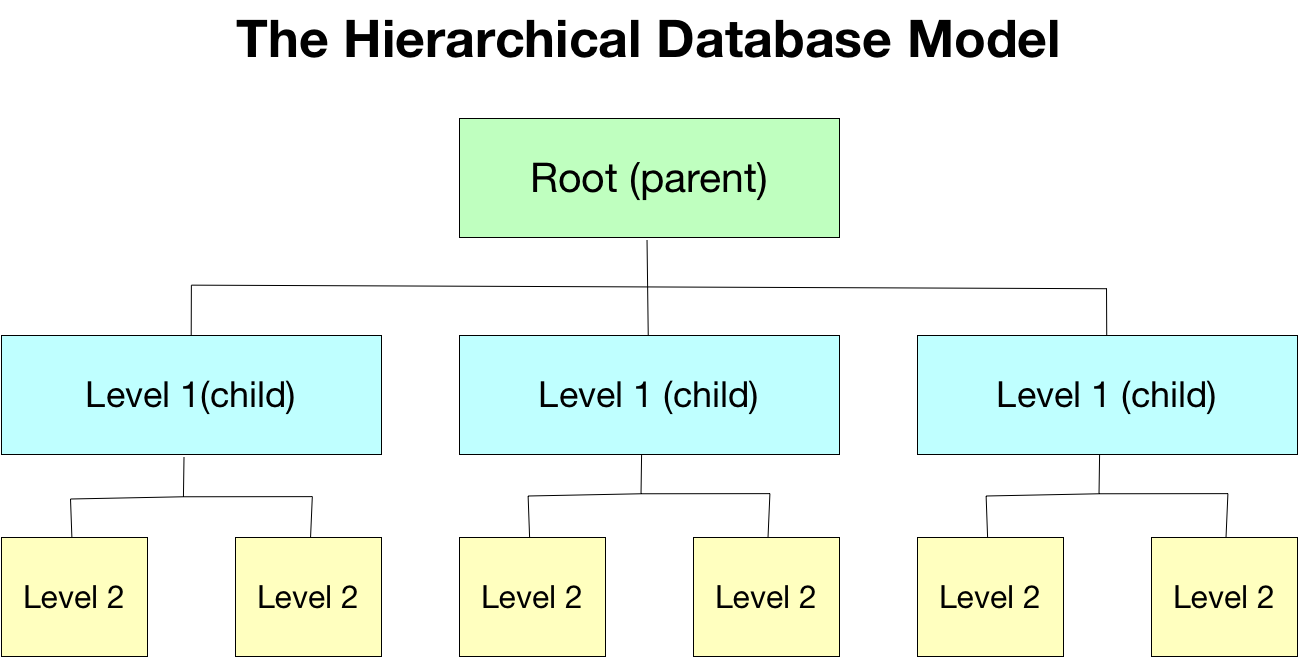
\includegraphics[scale=0.22]{./images/3-hierarchical-model}
			\caption{Hierarchical Model}
			\label{hier_model}
		\end{figure}
	\end{center}
	}
	
	\item {\textbf{Network model:} In 1969 a new model was announced that solved some of the limitations from the hierarchical model, which is that each node can be related with another node from the tree even if it isn’t from the same branch. Even if this model offered improvements it wasn’t massively used as IBM continued developing its products with the hierarchical model.
	\begin{center}
		\begin{figure}[h!]
			\centering
			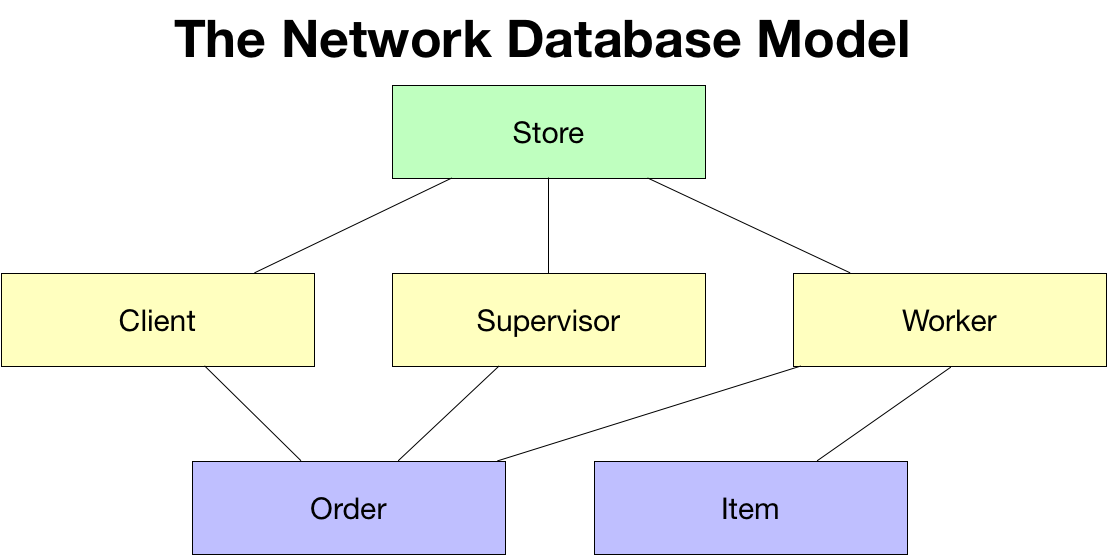
\includegraphics[scale=0.25]{./images/3-network-model}
			\caption{Network Model}
			\label{net_model}
		\end{figure}
	\end{center}
	}
	\item {\textbf{Relational model:} This model was easier to understand, and the programming interface was better. The problem was that when this model came to light, at the same time as the network model, it couldn’t be used due to limiting computer power, this in the 1980s was overcome by breakthroughs in the computing industry.\\
	This model differs from the other two models as it uses tables to store data, this data can be related with other tables making it a very attractive solution and making it easier to maintain.\\
	There are three ways of relating data in this model:
	\begin{itemize}
		\item {One-to-One}
		\item {One-to-Many}
		\item {Many-to-Many}
	\end{itemize}
	\begin{center}
		\begin{figure}[h!]
			\centering
			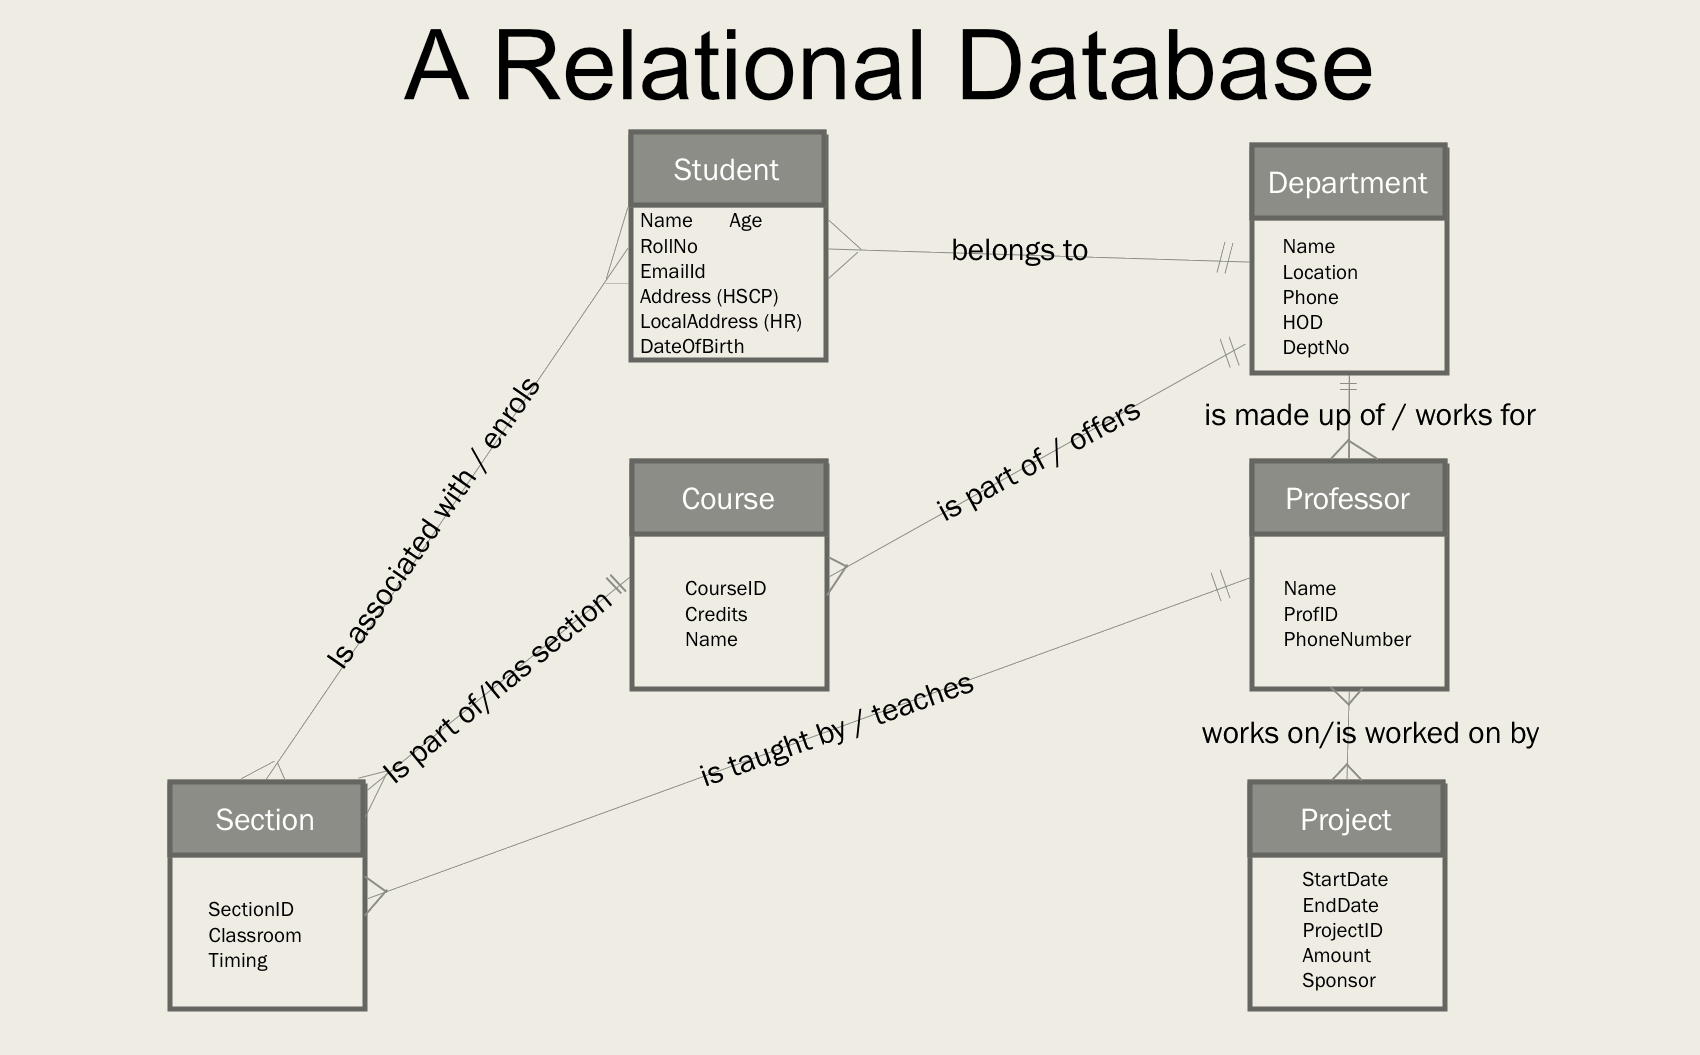
\includegraphics[scale=0.20]{./images/3-relational-model}
			\caption{Relational Model}
			\label{rel_model}
		\end{figure}
	\end{center}
	The language this model used is called Structured Query Language (SQL), there are several variations to this language depending on the application being used. Soon this became the standard and started being used in enterprise environments. In the mid-1990s a revolution in the development came about and new open sourced software with no cost for the developer started getting traction and with it the open source project of MySQL, which first version was developed by a Swedish company. The fact it was free, lowered the entry barrier for new developments.
	}
	\item {\textbf{NoSQL:} In 1998 a new term was created, NoSQL that categorized all databases that didn’t follow the same language as the most common relational databases. They came about with the internet boom, this was because a shift was coming around and more and more data was being ingested by the database. SQL databases have a harder time scaling up, with more demand in internet traffic and speed becoming the focus on the server-side, new ways of storing data had to be developed. It focuses more in simplicity and maintenance as it is easier to add new fields to existing data. 
	\begin{center}
		\begin{figure}[h!]
			\centering	
			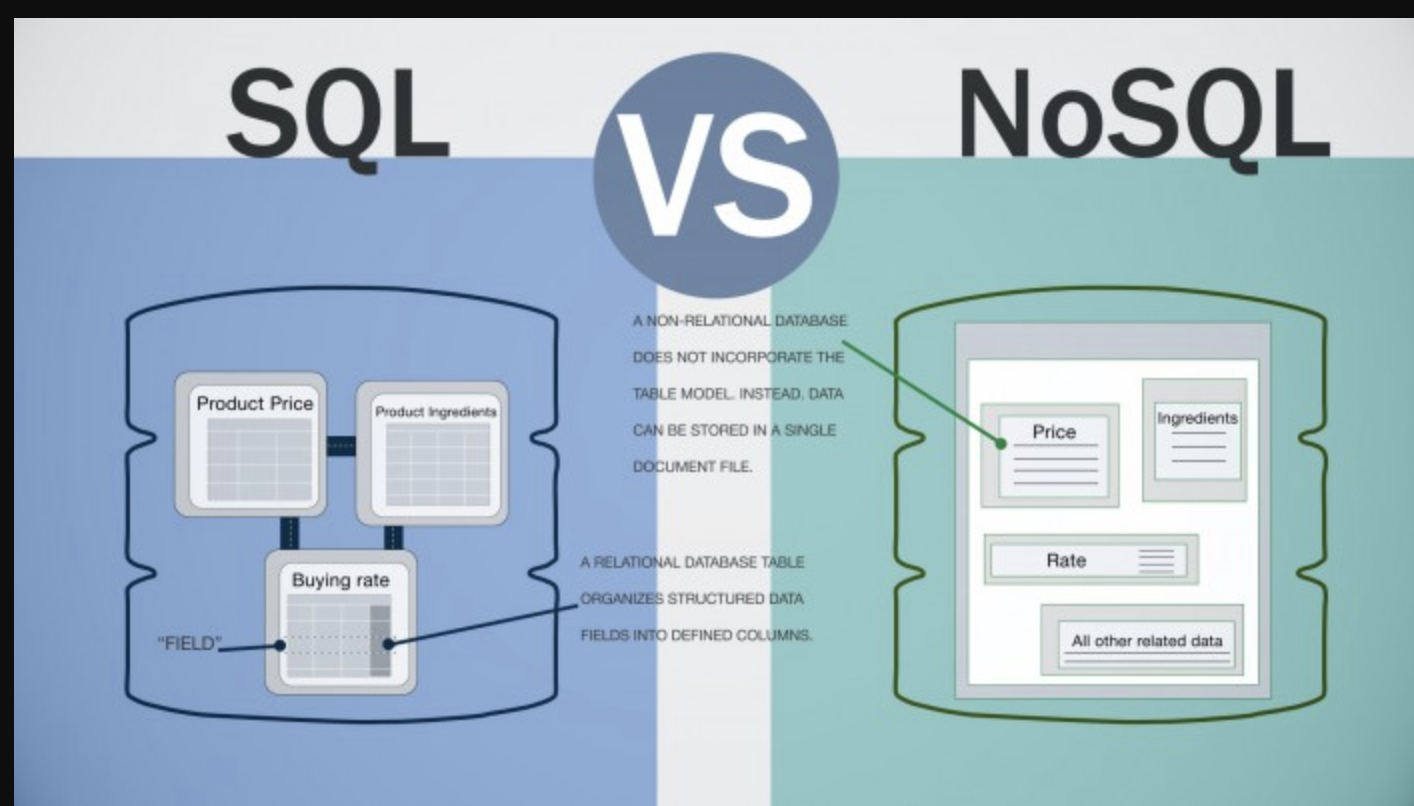
\includegraphics[scale=0.31]{./images/3-nosql}
			\caption{SQL vs NoSQL}
			\label{nosql}
		\end{figure}
	\end{center}
	Big Data has played a major role in the last few years, with storage prices in decline and the affordability of storing large amounts of data, has allowed scientists to analyze data to extract relevant information. This data is not only structured, created using applications or employees, it is data that can be extracted from unstructured sources. This can be comments from people on a product or if a media campaign is causing any impact. This information is highly valuable and that is why companies are so invested in it.\cite{db-hist}
	}
\end{itemize}
\clearpage
\subsection{Solutions}\label{sec:chap3_db_sol}
In this section we will expand on some of the solutions available for SQL and NoSQL databases.

\subsubsection{NoSQL}\label{sec:chap3_db_nosql}
This are some of the solutions for NoSQL databases, there is also on-premises or cloud databases that can be used.

\begin{table}[h!]
	\centering
	\setlength{\arrayrulewidth}{1.5pt}
	\resizebox{\linewidth}{!}{
		\begin{tabular}{|l|l|}
			\hline
			\rowcolor[HTML]{C0C0C0} 
			Name            & Description                                                                                                                                                                                                         \\ \hline
			\rowcolor[HTML]{96FFFB} 
			\multicolumn{2}{|c|}{\cellcolor[HTML]{96FFFB}On-Premise}                                                                                                                                                                              \\ \hline
			MongoDB         & \begin{tabular}[c]{@{}l@{}}Most\\ popular database, uses json-like documents to store data, which makes it much\\ more expressive.\end{tabular}                                                                     \\ \hline
			Redis           & \begin{tabular}[c]{@{}l@{}}An open-source, distributed database that uses key-value to store\\   data which makes it very fast to extract data.\end{tabular}                                                        \\ \hline
			Cassandra       & \begin{tabular}[c]{@{}l@{}}Open-source database created by Facebook with the focus on scalability\\   and high availability.\end{tabular}                                                                           \\ \hline
			\rowcolor[HTML]{96FFFB} 
			\multicolumn{2}{|c|}{\cellcolor[HTML]{96FFFB}Cloud}                                                                                                                                                                                   \\ \hline
			\rowcolor[HTML]{9B9B9B} 
			\multicolumn{2}{|c|}{\cellcolor[HTML]{9B9B9B}AWS}                                                                                                                                                                                     \\ \hline
			DynamoDB        & \begin{tabular}[c]{@{}l@{}}Key-value and document database that offers high scalability with database\\   management automated.\end{tabular}                                                                        \\ \hline
			DocumentDB      & \begin{tabular}[c]{@{}l@{}}Compatible with MongoDB, offers high performance, it has the compute\\   and storage elements separated to have more flexibility on scaling the\\   database.\end{tabular}               \\ \hline
			\rowcolor[HTML]{9B9B9B} 
			\multicolumn{2}{|c|}{\cellcolor[HTML]{9B9B9B}Microsoft Azure}                                                                                                                                                                         \\ \hline
			CosmosDB        & \begin{tabular}[c]{@{}l@{}}Azure solution that allows the use of different NoSQL models with the\\   functionality of scaling dynamically across the globe.\end{tabular}                                            \\ \hline
			\rowcolor[HTML]{9B9B9B} 
			\multicolumn{2}{|c|}{\cellcolor[HTML]{9B9B9B}Google Cloud}                                                                                                                                                                            \\ \hline
			Bigtable        & \begin{tabular}[c]{@{}l@{}}A very low latency solution that like other solutions focuses mainly\\   on scalability and availability. Allows easy integration with big data tools.\end{tabular}                      \\ \hline
			Cloud Firestore & \begin{tabular}[c]{@{}l@{}}Offers high availability with data replication, more expensive solution\\   than Bigtable, the main difference is that it offers better functionality for\\   transactions.\end{tabular} \\ \hline
	\end{tabular}}
	\label{nosql_tab}
	\caption{NoSQL Solutions}
\end{table}



\clearpage
\subsubsection{SQL}\label{sec:chap3_db_sql}
There are solutions both for on premises and cloud, some use the same language while others offer their own language.

\begin{table}[h!]
	\centering
	\setlength{\arrayrulewidth}{1.5pt}
	\resizebox{\linewidth}{!}{
		\begin{tabular}{|l|l|}
			\hline
			\rowcolor[HTML]{C0C0C0} 
			Name               & Description                                                                                                                                                                                           \\ \hline
			\rowcolor[HTML]{96FFFB} 
			\multicolumn{2}{|c|}{\cellcolor[HTML]{96FFFB}On-Premise}                                                                                                                                                                   \\ \hline
			MySQL              & \begin{tabular}[c]{@{}l@{}}The\\ most popular open-source SQL database.\end{tabular}                                                                                                                  \\ \hline
			PostgreSQL         & \begin{tabular}[c]{@{}l@{}}Focused more on the enterprise side, it offers higher extensibility than\\   MySQL.\end{tabular}                                                                           \\ \hline
			Oracle             & \begin{tabular}[c]{@{}l@{}}Offers the full service, but comes at a high price, used more by big enterprises\\   that can’t risk security mismanagement.\end{tabular}                                  \\ \hline
			\rowcolor[HTML]{96FFFB} 
			\multicolumn{2}{|c|}{\cellcolor[HTML]{96FFFB}Cloud}                                                                                                                                                                        \\ \hline
			\rowcolor[HTML]{9B9B9B} 
			\multicolumn{2}{|c|}{\cellcolor[HTML]{9B9B9B}AWS}                                                                                                                                                                          \\ \hline
			RDS                & \begin{tabular}[c]{@{}l@{}}Amazons own relational database solution, it offers a platform available\\   with different database engines such as MySQL, PostgreSQL, Oracle and many more.\end{tabular} \\ \hline
			Aurora             & A database engine that focuses on a higher throughput and scalability.                                                                                                                                \\ \hline
			\rowcolor[HTML]{9B9B9B} 
			\multicolumn{2}{|c|}{\cellcolor[HTML]{9B9B9B}Microsoft Azure}                                                                                                                                                              \\ \hline
			Azure SQL Database & Their own proprietary solution for a cloud database.                                                                                                                                                  \\ \hline
			Azure Database     & A solution compatible with existing SQL engines such as MySQL or PostgreSQL.                                                                                                                          \\ \hline
			\rowcolor[HTML]{9B9B9B} 
			\multicolumn{2}{|c|}{\cellcolor[HTML]{9B9B9B}Google Cloud}                                                                                                                                                                 \\ \hline
			Cloud SQL          & \begin{tabular}[c]{@{}l@{}}A google platform to use with database engines such as PostgreSQL or\\   MySQL.\end{tabular}                                                                               \\ \hline
			Cloud Spanner      & Solution that combines SQL elements with NoSQL.                                                                                                                                                       \\ \hline
	\end{tabular}}
	\label{sql_tab}
	\caption{SQL Solutions}
\end{table}


\section{Raspberry Pi}\label{sec:chap3_rasp}
A raspberry pi is a small single board computer with very low power consumption. Although limited in computing power its processor is still capable of running many programs and with recent models the hardware as gotten more powerful while maintaining its low price.\\

\begin{center}
	\begin{figure}[h!]
		\centering
		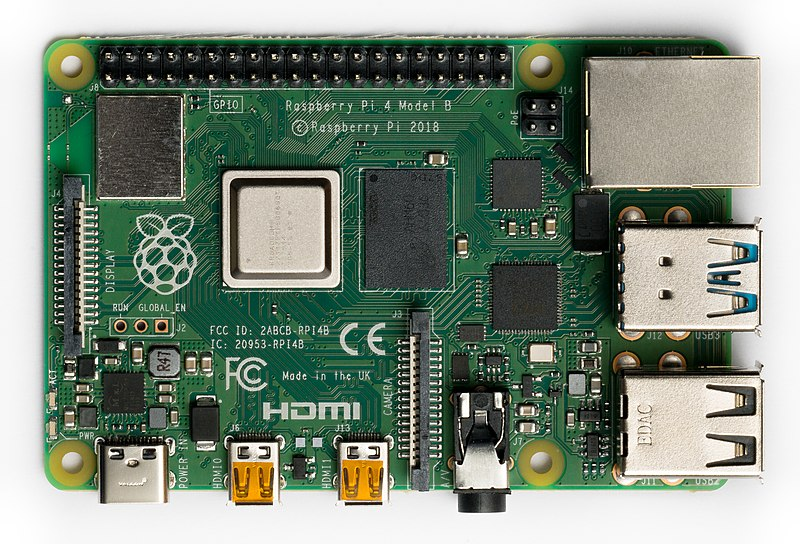
\includegraphics[scale=0.32]{./images/3-rasp-4}
		\caption{Raspberry Pi 4B}
		\label{rasp}
	\end{figure}
\end{center}

The Raspberry Pi has an ARM architecture processor which even though it benefits the pc on its low power requirements, it has compatibility issues with some software that is built for the x86 x64 processors.

The Raspberry Pi has many uses and as an affordable pc, here is a list of some examples to show the potential this device has, the limit to what you can do with a low powered computer are up to the developer’s imagination.

\begin{itemize}
	\item {\textbf{Media center:} You can configure the Raspberry Pi to act as a place to store or load films to watch on the users tv.}
	\item {\textbf{Retro gaming machine:} It can be used to remember old retro games by using the Raspberry Pi as an emulator for old games.}
	\item {\textbf{Game streaming:} Another option is using it as a device for games, streaming from the pc to the tv.}
	\item {\textbf{Security camera:} As it has an IO interface the developer can add modules like cameras and us it for surveillance to keep a house safe or check on the baby.}
	\item {\textbf{Home automation:} Having access to the local network the Raspberry Pi can be used as the brains of the house and use it to check data on the temperature, turn the heating on and plenty more.}
	\item {\textbf{Server:} The Raspberry Pi can also be used as a server, although limited in computing power it still has capability to be used for projects or as a development server.}
\end{itemize}

\subsection{Clusters}\label{sec:chap3_clusters}
A cluster is a set of computers that are tightly or loosely connected to work with each other, it acts like a single system, using the different computers to balance the load or for specific tasks.\\
For more intense projects these clusters may be required, the advantage the raspberry pi has is that its affordable price and small size factor the developer can build a powerful system with them. It can be used to balance the load on a web server. It can also be used as a mini supercomputer by supporting large amounts of cores and a large amount of RAM memory.

\section{Cloud Services}\label{sec:chap3_cloud}

Originally every company that wanted to manage their data and applications had to have a on-premises server to manage it, this required technical people having to be hired for the maintenance and upgrades the server required, when a company’s business model isn’t related to servers this becomes a burden. Another issue this causes is if not enough money is invested on this the availability of the server would be bad, and if it had to offer services in different countries latency becomes an issue.\\

Cloud computing offers a solution to these issues, a company can custom select what type of system they need to build their infrastructure, this can adapt to the companies needs in relation to processing power or storage space, this means that if a company focuses in the storage and transfer business they can build an infrastructure that focuses more on capacity, transfer speed and storage speed, compared to another company that works with artificial intelligence that may need a more powerful computer and less storage  space. This becomes available thanks to the improvements on virtualization.

\subsection{Virtualization}\label{sec:chap3_vir}

\begin{center}
	\begin{figure}[h!]
		\centering
		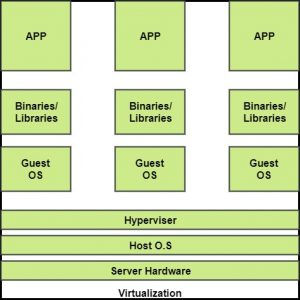
\includegraphics[scale=1]{./images/3-cloud-vir}
		\caption{Virtualization System}
		\label{cloud_vir}
	\end{figure}
\end{center}

Virtualization is a technique that separates the physical layer from the service level, this allows that a computer with certain resources have several virtual operating systems on top with different resources allocated. This offers many benefits in relation to cloud computing.

\begin{itemize}
	\item{Dynamic allocation of resources}
	\item{Lower costs of infrastructure}
	\item{Rapid scalability and remote access}
	\item{Multiple parallel OS}
	\item{Pay for time resources used}
\end{itemize}

There are different types of virtualization for different parts of the computer:

\begin{itemize}
	\item{\textbf{Storage virtualization:} This allows several servers storage as a single system, this virtualization allows it to be redundant as it offers tools for data replication and recovery, so if a server fails or a hard drive gets damaged the data remains intact.}
	\item{\textbf{Desktop virtualization:} This virtualization allows the user of the virtual system to access it remotely without knowing in what machine the OS is located.}
	\item{\textbf{Network virtualization:} The ability to create virtual networks to connect different elements in the data center allows different services to be able to communicate with each other.}
	\item{\textbf{Application virtualization:} With this type of virtualization different versions of a same application can coexist and allows an application to run without being installed in the traditional way or be supported by an OS.}
\end{itemize}

\subsection{Providers}\label{sec:chap3_prov}

\begin{itemize}
	\item{\textbf{AWS:} Amazon Web Services launched on 2006 and pioneered the business model for on-demand cloud computing, it has the highest market share of all the providers available. It offers a very large selection of products to choose from, making it better to create a well-defined architecture. AWS focuses more in the public cloud making enterprises with their own data center hard to interoperate with AWS.}
	\item{\textbf{Google Cloud:} The underdog in the competition between AWS and Microsoft Azure, it doesn’t have an enterprise focus which makes it harder to attract enterprise clients. It provides services with deep learning and machine learning which google cloud has leading technology.}
	\item{\textbf{Microsoft Azure:} A close competitor from Amazon Web Services, with years of experience and close relations with many enterprises Microsoft Azure offers what these clients want, that is to operate Azure functionality mixed with their own data center, allowing for a hybrid cloud.}
\end{itemize}

\section{Testing}\label{sec:chap3_test}

Testing is an essential part of software development which allows code to be bug free, even though it may seem tedious at the beginning in the long run it pays off and other developers will appreciate a built testing infrastructure.\\
There are several types of testing:\cite{testing}

\begin{itemize}
	\item {\textbf{Unit tests:} These are the lowest level of testing, where individual methods and functions are tested to verify that they are working correctly. Unit tests are easy to automate and are quite common in continuous integration, where in every new build it verifies that anything previous is working correctly.}
	\item {\textbf{Integration tests:} These tests are higher level where different modules or services work well with each other. The complication of running these tests is that it requires certain parts of the application to be running.}
	\item {\textbf{Functional tests:} Focusing more on the business requirements, these tests only are interested in the result not the middle steps between starting the action and the result. It differentiates from integration testing is that integration tests are only interested in checking if the system works and functional testing is more interested in verifying that the result is correct.}
	\item {\textbf{End-to-end tests:} End-to-end testing simulates user behavior to test if the flows of the application are working correctly. It is a very high level of testing and it is more complicated to automate due to needing interaction directly with the application, this interaction if automated needs to be maintained because any update on the interface of the application can render the test useless.}
	\item {\textbf{Performance testing:} This type of tests is very important to have when building big applications as it provides relevant information on how scalable the application is and if any significant latency or crashes are noticed.}
	\item {\textbf{Smoke testing:} Like functional tests but less expensive, just to verify the main systems are operational, if the deployment is functional then more expensive tests can be run.}
\end{itemize}

\subsection{Automation}\label{sec:chap3_auto}

Having a person run the tests above is possible but it would be very expensive, counter-productive and a very boring job as they must run every time a deployment or a new feature is added. To automate the tests programmatically the developer needs a testing framework that suits the application. These frameworks are dependent of the programming language used. Even though this automation allows to execute tests to verify the application the next step is to whenever the developer chooses to deploy the application, the tests run automatically before deploying, this is called continuous integration.

	\chapter{Solution Proposed}\label{chap:4}

\section{Architecture}\label{sec:chap4_arch}

[INSERT FIGURE OF ARCHITECTURE]

\subsection{Hardware}\label{sec:chap4_arch_hard}

\subsection{Software}\label{sec:chap4_arch_soft}

\section{Network-Based Mobility Solution}\label{sec:chap4_net_based}

\subsection{Attachment}\label{sec:chap4_net_based_attach}

\subsection{Start video}\label{sec:chap4_net_based_video}

\subsection{Intradistrict handover}\label{sec:chap4_net_based_intra}

\subsection{Interdistrict handover}\label{sec:chap4_net_based_inter}

\section{Host-Based Mobility Solution with LTE emulation}\label{sec:chap4_host_based}

\subsection{Handover to LTE district}\label{sec:chap4_host_based_lte}

\section{On-demand Infrastructure}\label{sec:chap4_ondemand}

\subsection{Switching off an Access Point}\label{sec:chap4_host_based_lte}

\subsection{Switching on an Access Point}\label{sec:chap4_host_based_lte}




	\chapter{Planning and Budget}\label{chap:8}
\section{Planning}\label{sec:chap5_plan}
The original plan was to develop the whole project in five months in two different stages and documenting the whole process, the first stage was programmed to las two weeks designing and thinking on the objective of the application and making sure that the idea is viable before writing a line of code with a form sent to possible users. The next stage was the development step, first creating the tests that will confirm the application works correctly, this stage was predicted to last 4 months. The following steps can be seen in the Gantt graph on the next page.\\

After the five months of development, due to external factors, the project was seriously delayed and a redesign had to be done as the complexity of the context manager in the original design made it unviable to deliver for this year. This made it necessary to rethink how to adapt the project to reach the target of September for delivery. In order to reach the objective an extension on the different parts of the project have to be done, this included two more weeks of planning and preparation, twelve more weeks of development where the new configuration and implementation was completed, the rest of the extension was filling out the documentation with the new design.\\

Even though this was a setback to the project, it allowed gaining experience in how the perception of time in completing tasks has to be refined in order to avoid overextending a project and having inefficiencies.

\begin{landscape}
	

\begin{ganttchart}[
	canvas/.append style={fill=none, draw=black!5, line width=.75pt},
	hgrid style/.style={draw=black!5, line width=.75pt},
	vgrid={*1{draw=black!5, line width=.75pt}},
	title/.style={draw=none, fill=none},
	title label font=\bfseries\footnotesize,
	title label node/.append style={below=1pt},
	include title in canvas=false,
	bar label font=\mdseries\small\color{black!70},
	bar label node/.append style={left=2cm},
	y unit chart=0.9cm,
	bar/.append style={draw=none, fill=barblue},
	bar progress label font=\mdseries\footnotesize\color{black!70},
	group/.append style={draw=none, fill=groupblue},
	group left shift=0,
	group right shift=0,
	group height=.5,
	group peaks tip position=0,
	group label node/.append style={left=.6cm},
	group progress label font=\bfseries\small,
	]{1}{25}
	\gantttitle[
	title label node/.append style={below left=1pt and 0pt}
	]{WEEKS:\quad1}{1}
	\gantttitlelist{2,...,25}{1} \\
	\ganttgroup{Project design}{1}{2} \\
	\ganttbar{Use cases}{1}{1} \\
	\ganttbar{Viability analysis}{1}{2} \\
	\ganttbar{State of the art analysis}{1}{2} \\
	\ganttbar{Choose what resources to use}{2}{2} \\
	\ganttbar{System design}{2}{2} \\[grid]
	\ganttgroup{Project development}{2}{16} \\
	\ganttbar{Tests}{2}{3} \\
	\ganttbar{Webhook}{3}{4} \\
	\ganttbar{Controller}{4}{6} \\
	\ganttbar{Context manager}{7}{11} \\
	\ganttbar{Activity manager}{11}{16} \\[grid]
	\ganttgroup{Process Documentation}{2}{20} \\
	\ganttbar{Memory redaction}{2}{17} \\
	\ganttbar{Presentation}{18}{20}
	\end{ganttchart}

\end{landscape}


	
%	\begin{ganttchart}[
%		canvas/.append style={fill=none, draw=black!5, line width=.75pt},
%		hgrid style/.style={draw=black!5, line width=.75pt},
%		vgrid={*1{draw=black!5, line width=.75pt}},
%		title/.style={draw=none, fill=none},
%		title label font=\bfseries\footnotesize,
%		title label node/.append style={below=1pt},
%		include title in canvas=false,
%		bar label font=\mdseries\small\color{black!70},
%		bar label node/.append style={left=2cm},
%		y unit chart=0.9cm,
%		bar/.append style={draw=none, fill=barblue},
%		bar progress label font=\mdseries\footnotesize\color{black!70},
%		group/.append style={draw=none, fill=groupblue},
%		group left shift=0,
%		group right shift=0,
%		group height=.5,
%		group peaks tip position=0,
%		group label node/.append style={left=.6cm},
%		group progress label font=\bfseries\small,
%		]{1}{16}
%		\gantttitle[
%		title label node/.append style={below left=1pt and 0pt}
%		]{WEEKS:\quad1}{1}
%		\gantttitlelist{2,...,16}{1} \\
%		\ganttgroup{Project design}{1}{2} \\
%		\ganttbar{Change resources}{1}{2} \\
%		\ganttbar{New system design}{2}{2} \\[grid]
%		\ganttgroup{Project development}{3}{12} \\
%		\ganttbar{Pipeline design}{3}{4} \\
%		\ganttbar{Story elaboration}{4}{6} \\
%		\ganttbar{Custom activities}{7}{10} \\
%		\ganttbar{Activity manager}{10}{12} \\[grid]
%		\ganttgroup{Process Documentation}{2}{16} \\
%		\ganttbar{Memory redaction}{2}{14} \\
%		\ganttbar{Presentation}{15}{16}
%	\end{ganttchart}
	
\section{Budget}\label{sec:chap5_budg}

In this section, we will explain the budget for the project, which contains the resources used when developing the project. Below is a table with all the details about the cost for the hardware, software and human resources.\\

\begin{table}[h!]
	\centering
	\setlength{\arrayrulewidth}{1.5pt}
	\resizebox{\linewidth}{!}{
	\begin{tabular}{|r|r|r|r|r|r|r|} 
		\hline
		\multicolumn{7}{|c|}{{\cellcolor[rgb]{0.502,1,1}}Hardware}                                                                                                                              \\ 
		\hline
		\rowcolor[rgb]{0.753,0.753,0.753} \multicolumn{1}{|l|}{Name}                           &  \multicolumn{1}{l|}{Cost}                       &  \multicolumn{1}{l|}{Units} &  \multicolumn{1}{l|}{Duration(months)}                 &  \multicolumn{1}{l|}{\% use in project} &  \multicolumn{1}{l|}{Amortization(months)} &  \multicolumn{1}{l|}{Chargeable cost}   \\ 
		\hline
		
		 \multicolumn{1}{|l|}{Laptop}                                                           & 699 \euro                      & 1     & 9                        & 100 \%            & 48           & 131,07 \euro          \\ 
		\hline
		 \multicolumn{1}{|l|}{Raspberry Pi}                                                     & 35 \euro                       & 1     & 5                        & 55,55 \%          & 48           & 3,65 \euro            \\ 
		\hline
		 \multicolumn{1}{|l|}{Smartphone}                                                       & 560 \euro                      & 1     & 9                        & 100\%             & 36           & 140 \euro             \\ 
		\hline
		\multicolumn{5}{|r|}{{\cellcolor[rgb]{0,0.682,0.937}}Total:}                                                                                          & \multicolumn{2}{r|}{274,72 \euro}    \\ 
		\hline
		\multicolumn{7}{|c|}{{\cellcolor[rgb]{0.502,1,1}}Software}                                                                                                                              \\ 
		\hline
		\rowcolor[rgb]{0.753,0.753,0.753} \multicolumn{1}{|l|}{Name}                           & \multicolumn{1}{l|}{Cost}                       & \multicolumn{1}{l|}{Units} & \multicolumn{1}{l|}{Duration}                 & \multicolumn{1}{l|}{\% use in project} & \multicolumn{2}{l|}{Total cost}  \\ 
		\hline
		\begin{tabular}[l]{@{}l@{}} Azure virtual \\machine \end{tabular} & \textasciitilde{}10 \euro/month & 1     & 4                        & 44,45 \%          & \multicolumn{2}{r|}{40 \euro}        \\ 
		\hline
		\multicolumn{5}{|r|}{{\cellcolor[rgb]{0,0.682,0.937}}Total:}                                                                                          & \multicolumn{2}{r|}{40 \euro}        \\ 
		\hline
		\multicolumn{7}{|c|}{{\cellcolor[rgb]{0.502,1,1}}Human Resources}                                                                                                                       \\ 
		\hline
		\rowcolor[rgb]{0.753,0.753,0.753} \multicolumn{2}{|l|}{Category}                              & \multicolumn{2}{l|}{~ Cost/Hour} & Total hours       & \multicolumn{2}{l|}{Total cost}  \\ 
		\hline
		\multicolumn{2}{|l|}{Developer}                                                               & \multicolumn{2}{r|}{40 \euro/hour}   &  \multicolumn{1}{r|}{792}               & \multicolumn{2}{r|}{31.680 \euro}     \\ 
		\hline
		\multicolumn{2}{|l|}{Project Manager}                                                         & \multicolumn{2}{r|}{60 \euro/hour}   &  \multicolumn{1}{r|}{144}               & \multicolumn{2}{r|}{8.640 \euro}      \\ 
		\hline
		\multicolumn{5}{|r|}{{\cellcolor[rgb]{0,0.682,0.937}}Total:}                                                                                          & \multicolumn{2}{r|}{40.320 \euro}     \\
		\hline
		\multicolumn{5}{| r|}{{\cellcolor[rgb]{0.749,0.749,0.749}}Max Total:}                                                                                 & \multicolumn{2}{r|}{40.634,72 \euro}  \\
		\hline                                  
		\hline
		\multicolumn{5}{|r|}{{\cellcolor{yellow}}Total + Tax (21\%):}                                                                                       & \multicolumn{2}{r|}{49.268,02 \euro}  \\
		\hline
	\end{tabular}}
	\label{costs}
	\caption{Budget}
\end{table}

To give some context to the different parts of the table we will explain them further. Starting with the hardware the resources needed where a laptop for the development, the smartphone to test the app and the Raspberry Pi for the server, the reason for using the Raspberry Pi 55,5\% of the projects is due to the change in design mid project to use instead the Azure Virtual Machine as the new Server. The cost for the hardware is based on the cost of the product, and the amortization based on the average lifespan of these products.\\

For the software, the only software used was the virtual machine from azure. The reason the cost for the Azure Machine is relative is that it has a pricing system based on paying what you use, meaning that depending on how much you use the resources the pricing varies. For this project the price of usage at the moment of writing this memory has been 40 \euro \space as virtual machine was used only when required to minimize costs.\\

The human resources used in the project were where most of the budget of the project went to, the hourly rate is based on similar projects done and by the knowledge of people in the industry. The developer works 4 hours a day in average on the project for the length of the project considering only working days. For the project manager he works only 5,5 days out of the 22 working days in a month, to control that the project is on track and make adjustments to it.\\

Based on all these costs the total budget for the project is FORTY NINE THOUSAND TWO HUNDRED NINETY EIGHT AND TWO CENTS EUROS.
 in the case of this project the virtual machine was used only when required to minimize costs.

	%\chapter{Socioeconomic Environment}\label{chap:8}


	\chapter{Conclusions}\label{chap:11}


	
	\bibliographystyle{ieeetr}
\bibliography{main}

		
	\appendix

	


\end{document}
